

\section{Experimental design}


\subsection{Rationale for synthetic validation}

Real observations do not provide ground truth for regime boundaries or causal graphs.
This prevents direct measurement of recovery accuracy. Synthetic structural causal
models have known graphs and coefficients, so every output can be evaluated: regimes
with the Adjusted Rand Index, graphs against the generating DAG, effects against the
generating coefficients, and persistence against the true $\phi$.


\subsection{Generating process}

Two regimes of 5,000 observations are generated in temporal order and concatenated
without shuffling. The four spectral-state variables follow independent,
mean-reverting first-order autoregressive processes:

Equation~\eqref{eq:ch5-1} defines the mean-reverting process:
\begin{equation}
    \label{eq:ch5-1}
X(t) = \mu_X + \varphi\big(X(t-1) - \mu_X\big) + \epsilon_X(t), \qquad \varphi = 0.90
\end{equation}

with $\epsilon_X(t) \sim N(0, 0.10^2)$ for all four variables. The mean-reverting
form preserves the chosen mean from the first step. It therefore avoids the decay of
initial values and removes the need for a burn-in period.

The target variable is generated by Equation~\eqref{eq:ch5-2}:

\begin{equation}
    \label{eq:ch5-2}
\log F_R(t) = \mu_F + \phi\big(\log F_R(t-1) - \mu_F\big) + \sum_{v} \beta_v^{(z)}\big(X_v(t) - \mu_v\big) + \epsilon_F(t)
\end{equation}

with $\phi = 0.50$. The predictors are centred and $F_R$ is mean-reverting. Thus,
$\mathrm{E}[\log F_R] = \mu_F$ for any coefficient vector, so both regimes have the
same means.


\subsection{Why equal means are necessary for a valid test}

Equal means are necessary for a meaningful test. The Chow null hypothesis in
Equation~\eqref{eq:ch4-11} compares the full coefficient vectors, including the
intercept $w_0$. A mean shift would change the intercept and could cause rejection
without any change in the causal slopes. Structure-blind clustering would also benefit
from that level shift, making the baseline comparison uninformative.

With equal means, the regimes differ only in which variable has a non-zero coefficient
on $\log F_R$. A rejection can therefore reflect a mechanism change. Table~\ref{tab:ch5-distribution}
confirms the construction.



\begin{table}[htbp]
    \centering
    \small
    \caption{Distributional summary of the generated data}
    \label{tab:ch5-distribution}
    \begin{tabularx}{\textwidth}{|>{\raggedright\arraybackslash}X|>{\raggedright\arraybackslash}X|>{\raggedright\arraybackslash}X|>{\raggedright\arraybackslash}X|>{\raggedright\arraybackslash}X|}
        \hline
        Variable & Hard mean & Soft mean & Hard s.d. & Soft s.d. \\ \hline
        $\log L_X$ & 37.4931 & 37.4756 & 0.2332 & 0.2290 \\ \hline
        $\Gamma$ & 1.6124 & 1.5909 & 0.2347 & 0.2174 \\ \hline
        $\log T_{in}$ & 0.2934 & 0.3289 & 0.2188 & 0.2174 \\ \hline
        $HR$ & 0.7669 & 0.7320 & 0.2377 & 0.2297 \\ \hline
        $\log F_R$ & 27.9747 & 27.9595 & 0.3803 & 0.2289 \\ \hline
    \end{tabularx}
\end{table}

The means differ by less than 0.04 for every variable. The variance of $\log F_R$ is
still different (0.380 versus 0.229), because the Hard State has larger coefficient
magnitudes. This remaining difference is addressed in the baseline comparison.


\subsection{Ground-truth structures}



\begin{table}[htbp]
    \centering
    \small
    \caption{Generating coefficients}
    \label{tab:ch5-coefficients}
    \begin{tabularx}{\textwidth}{|>{\raggedright\arraybackslash}X|>{\raggedright\arraybackslash}X|>{\raggedright\arraybackslash}X|}
        \hline
        Coefficient & Hard State ($G_1$) & Soft State ($G_2$) \\ \hline
        $\beta_{L_X}$ & $+0.70$ & $+0.18$ \\ \hline
        $\beta_{\Gamma}$ & $-0.30$ & $+0.20$ \\ \hline
        $\beta_{T_{in}}$ & $0.00$ \textit{(isolated)} & $-0.40$ \\ \hline
        $\beta_{HR}$ & $-0.40$ & $0.00$ \textit{(isolated)} \\ \hline
        $\phi$ & $+0.50$ & $+0.50$ \\ \hline
    \end{tabularx}
\end{table}

The Hard State is interpreted as jet-dominated: radio emission is driven by X-ray
luminosity, photon index, and hardness ratio, while inner-disk temperature is isolated.
The Soft State is disk-dominated, with hardness ratio isolated instead.

The generating coefficients are listed in Table~\ref{tab:ch5-coefficients}.

The corresponding ground-truth causal structures are shown in Figure~\ref{fig:chapter5-2},
and the generated series and its true and discovered boundaries are shown in
Figure~\ref{fig:chapter5-3}.


\begin{figure}[htbp]
    \centering
    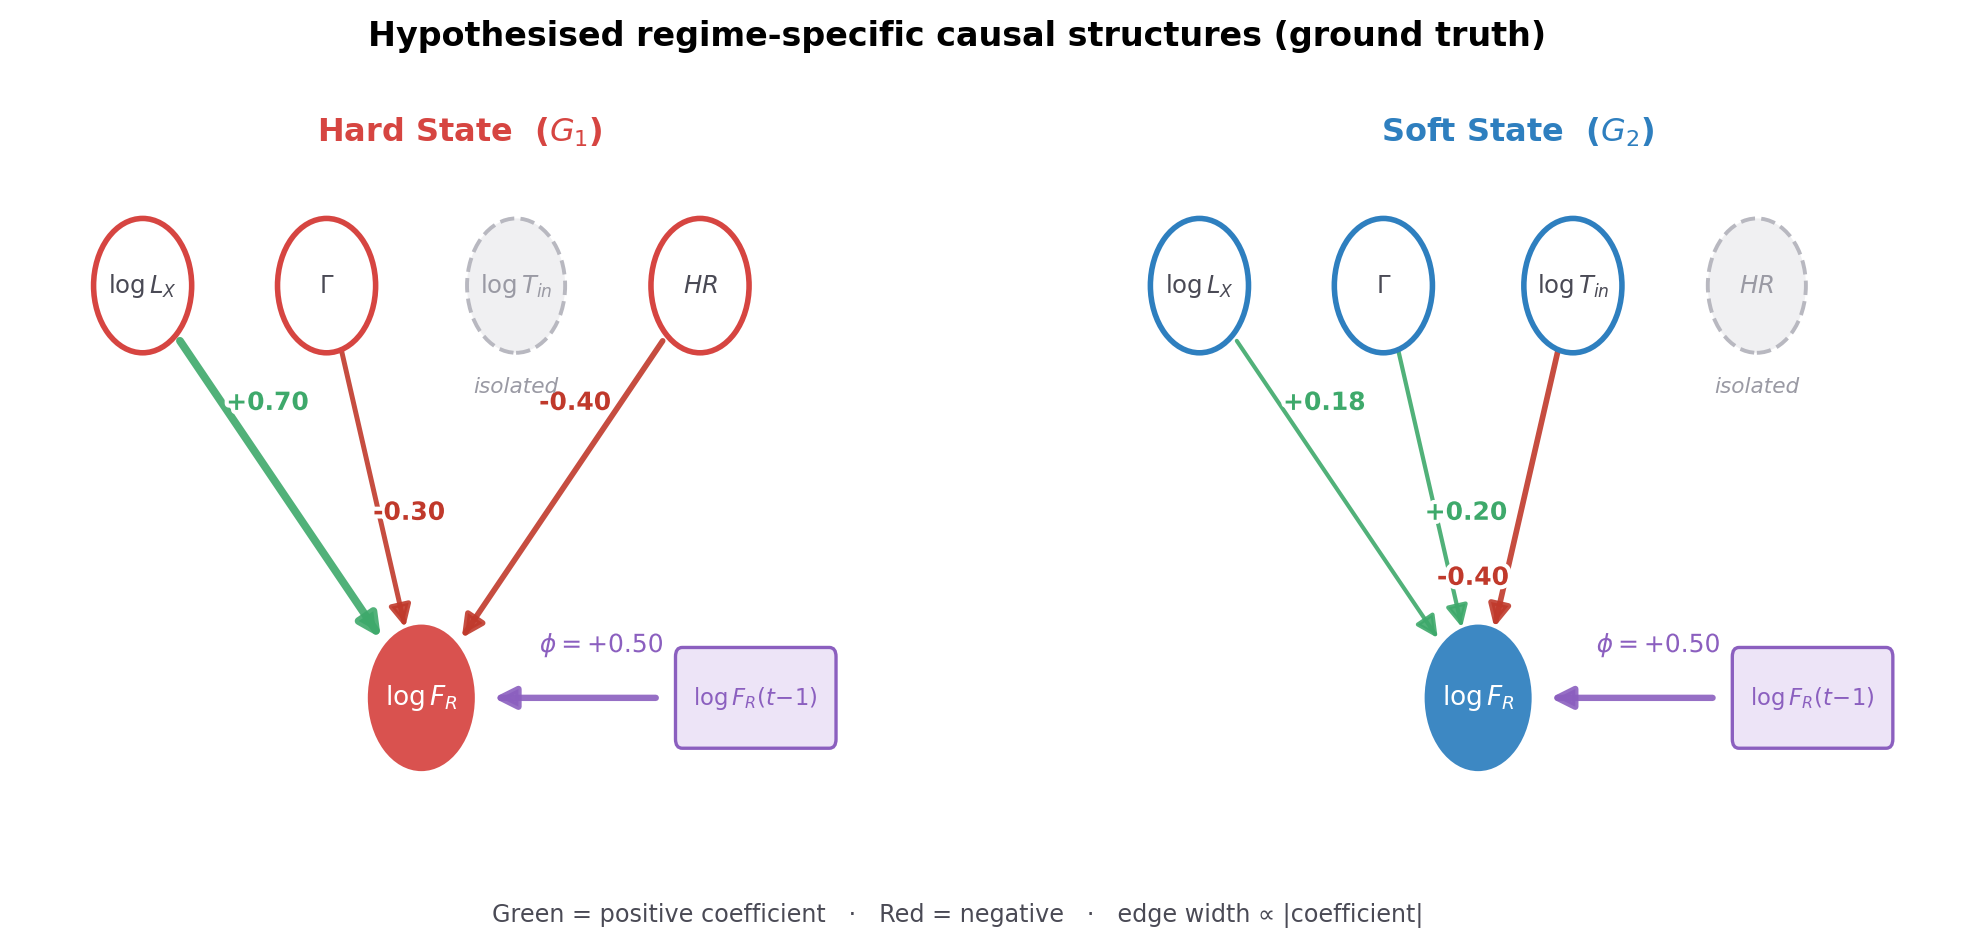
\includegraphics[width=\textwidth]{figs/fig02_ground_truth_dags.png}
\caption{Hypothesised regime-specific causal structures. Edge width is proportional to coefficient magnitude. The causally isolated variable in each regime is shown dashed.}
    \label{fig:chapter5-2}
\end{figure}

Figure~\ref{fig:chapter5-2} shows the causal structures used to generate the two
regimes. The Hard State contains edges from $L_X$, $\Gamma$, and $HR$ into $F_R$;
$T_{in}$ is isolated. In the Soft State, $T_{in}$ becomes a parent of $F_R$ and $HR$
is isolated. These mechanism changes are the target of regime discovery.


\begin{figure}[htbp]
    \centering
    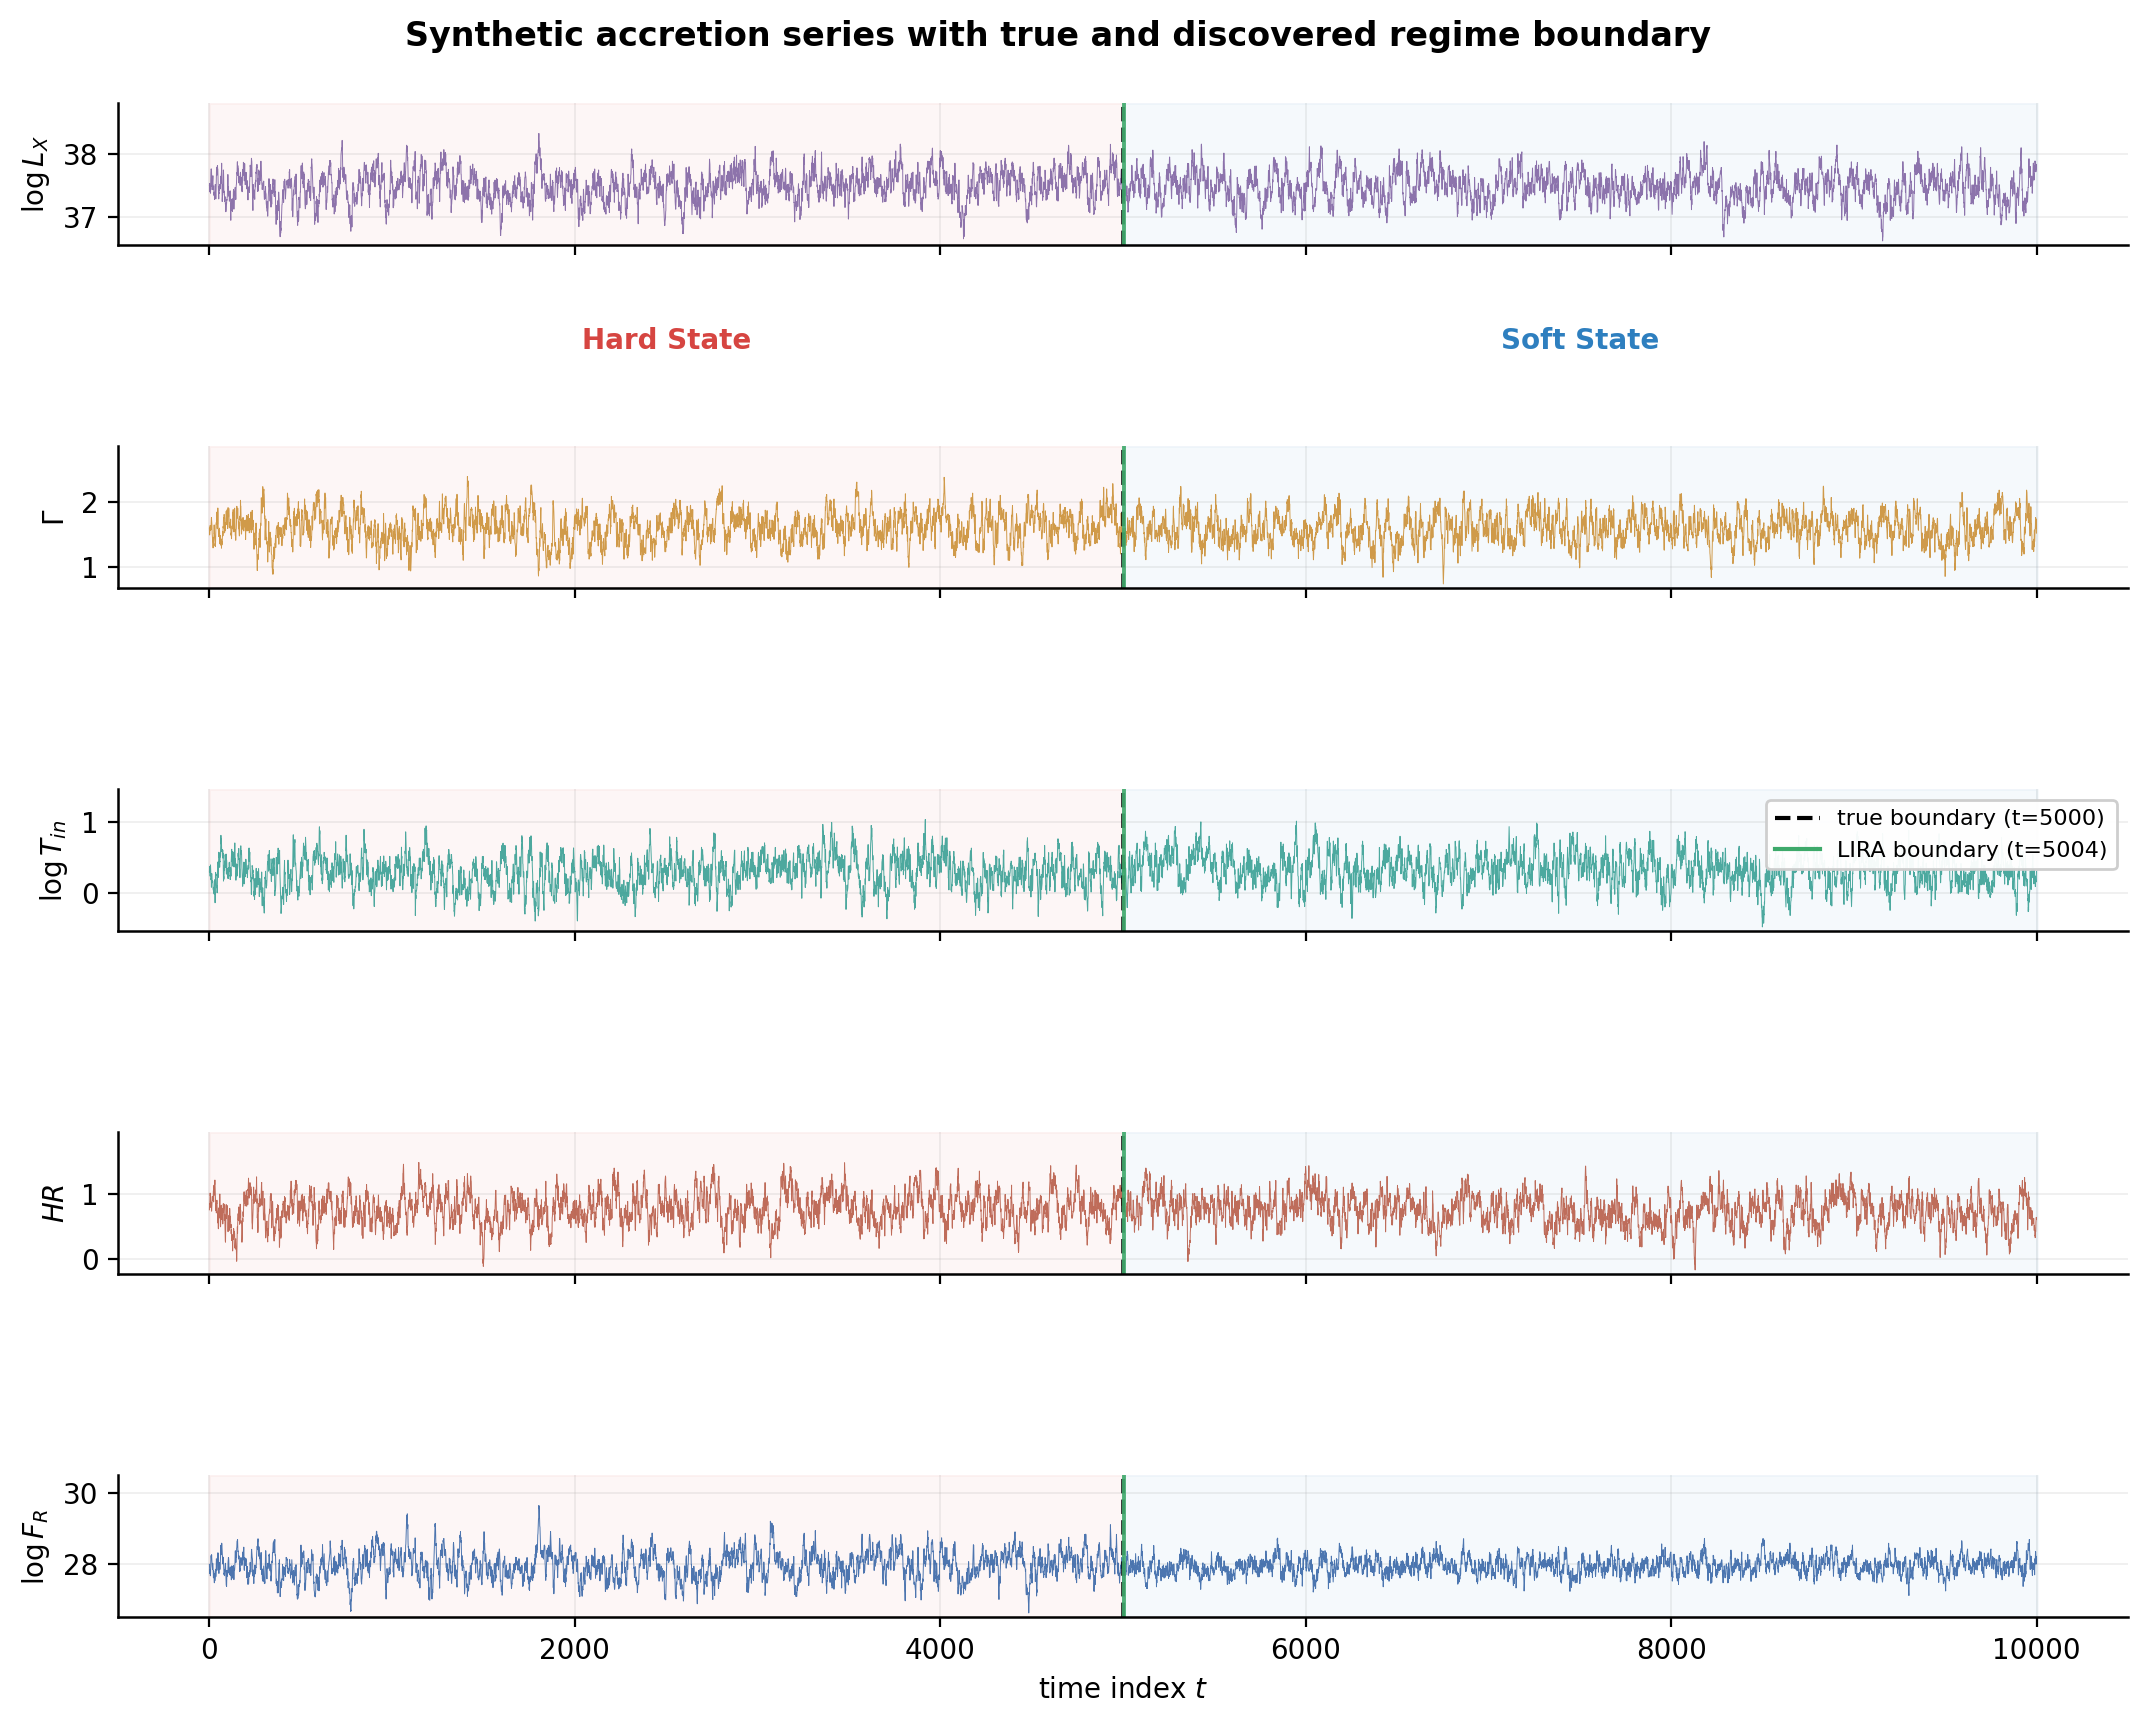
\includegraphics[width=\textwidth]{figs/fig03_timeseries.png}
\caption{The generated series with the true boundary (dashed) and the boundary discovered by LIRA (solid). No level shift is visible at the boundary in any variable, by construction.}
    \label{fig:chapter5-3}
\end{figure}

Figure~\ref{fig:chapter5-3} shows the generated series and the two boundaries. The
levels remain similar across the true boundary, so the regimes are not separated by
a simple mean shift. The recovered boundary is close to the generating boundary,
which supports the numerical localisation result in Section~5.3.1.


\section{Validation of the autoregressive extension}

Section~4.3.3 argues that the lag term is required for the Chow $F$ derivation to hold. This
is verified directly. Fitting the static specification in Equation~\eqref{eq:ch4-5} within the first regime
yields residuals with first-order autocorrelation $0.507$ and a Ljung--Box statistic at
10 lags of $1713.4$ ($p < 10^{-16}$), decisively rejecting independence. Fitting the
autoregressive specification in Equation~\eqref{eq:ch4-6} to the same data reduces the first-order residual
autocorrelation to $-0.011$, with a Ljung--Box statistic of $13.2$ ($p = 0.211$),
consistent with independence at any conventional level.

The residual-independence diagnostics are summarised in Table~\ref{tab:ch5-residuals}.



\begin{table}[htbp]
    \centering
    \small
    \caption{Residual independence diagnostics (Hard State segment)}
    \label{tab:ch5-residuals}
    \begin{tabularx}{\textwidth}{|>{\raggedright\arraybackslash}X|>{\raggedright\arraybackslash}X|>{\raggedright\arraybackslash}X|>{\raggedright\arraybackslash}X|>{\raggedright\arraybackslash}X|}
        \hline
        Specification & ACF(1) & Ljung--Box(10) & $p$ & Residuals i.i.d.? \\ \hline
        Static, Eq. (4.5) & $0.507$ & $1713.4$ & $<10^{-16}$ & rejected \\ \hline
        Autoregressive, Eq. (4.6) & $-0.011$ & $13.2$ & $0.211$ & not rejected \\ \hline
    \end{tabularx}
\end{table}

Table~\ref{tab:ch5-residuals} shows that the static model leaves strong residual
autocorrelation, while the AR(1) model produces residuals consistent with independence.
The corresponding autocorrelation plots are shown next.

\begin{figure}[htbp]
    \centering
    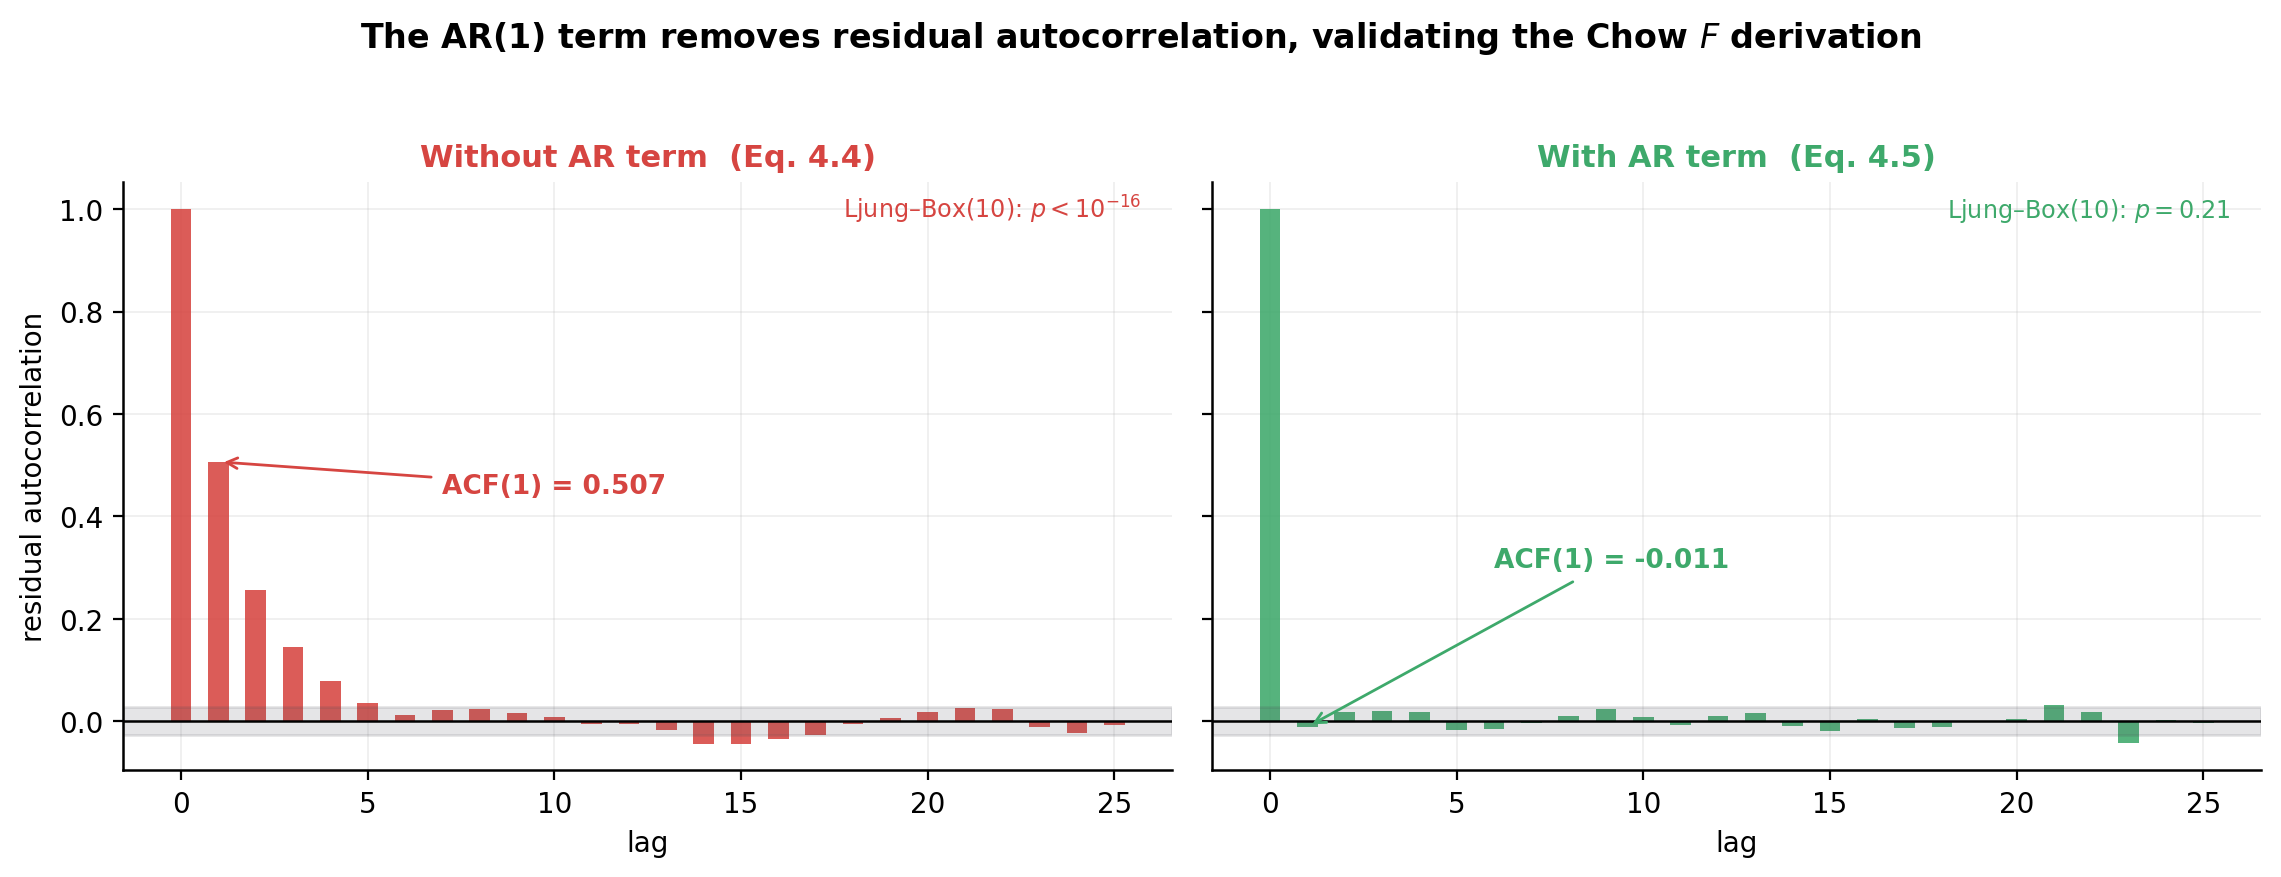
\includegraphics[width=\textwidth]{figs/fig06_residual_acf.png}
    \caption{Residual autocorrelation functions with and without the AR(1) term. Shaded band gives the 95\% interval under independence.}
    \label{fig:chapter5-6}
\end{figure}

The autoregressive specification therefore supports the distributional assumption in
Equation~\eqref{eq:ch4-15}, while the static specification does not. The lag term is
necessary, not merely beneficial.

Figure~\ref{fig:chapter5-6} shows the corresponding residual autocorrelation diagnostics.


\section{Regime discovery}


\subsection{Boundary localisation}

Figure~\ref{fig:chapter5-4} shows the lagged Chow statistic evaluated across all admissible split indices
at the root node. The statistic rises monotonically toward the true boundary and
attains its maximum of $F_{lag} = 963.4$ at $\tau^* = 5004$, against a true boundary at
$t = 5000$, a localisation error of four observations, or $0.04\%$ of the series
length. The associated $p$-value is below the limit of double-precision representation.


\begin{figure}[htbp]
    \centering
    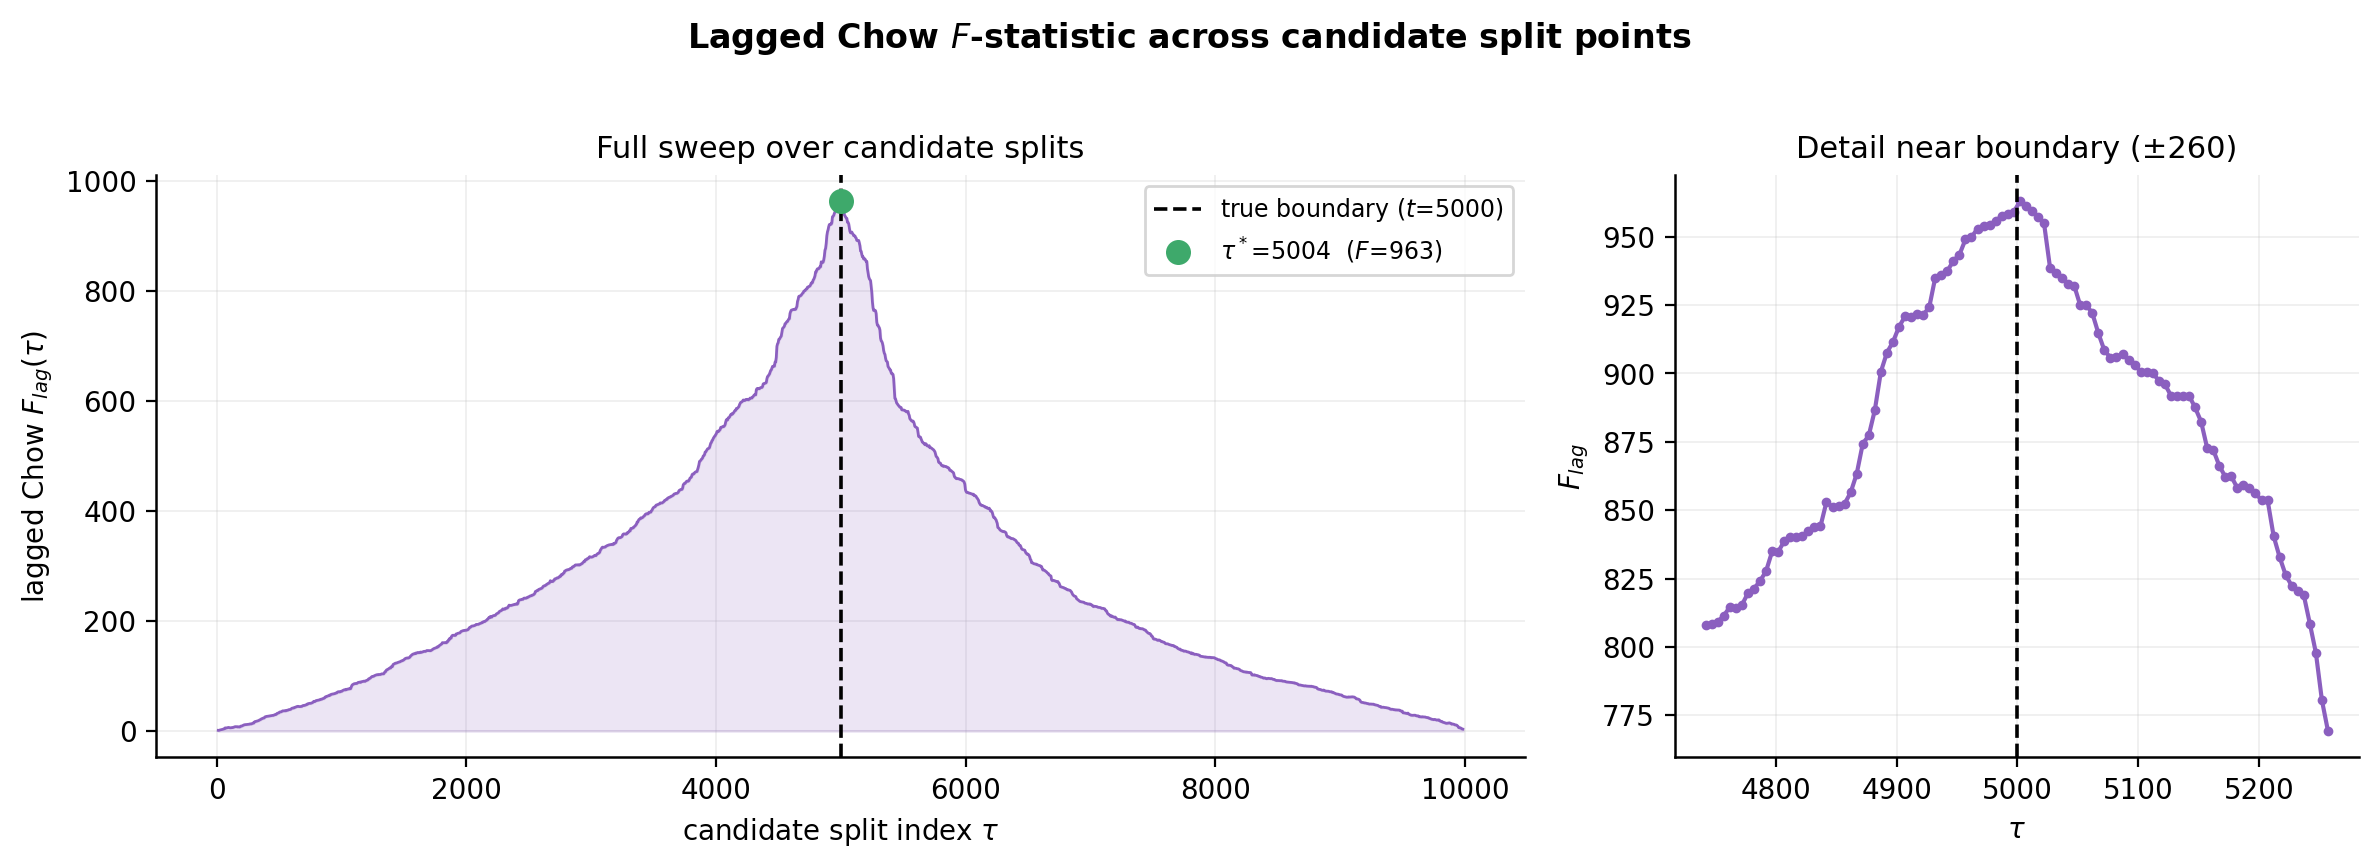
\includegraphics[width=\textwidth]{figs/fig04_chow_F_curve.png}
    \caption{Lagged Chow $F$-statistic across candidate split points, with detail near the boundary.}
    \label{fig:chapter5-4}
\end{figure}


\subsection{Operation of the two gates}

At the root node both gates are satisfied: $F_{lag} = 963.4$ with $p < 10^{-16}$, and
$BIC_1 = -41362$ against $BIC_2 = -45874$, so the split reduces BIC by $4512$ and is
accepted. Recursion then proceeds into each child.

At both child nodes the Chow test is significant: $F_{lag}=3.15$, $p=0.004$ on the
left and $F_{lag}=3.27$, $p=0.003$ on the right. A Chow-only procedure would have
created extra, spurious boundaries. BIC rejects both splits. The split increases BIC
by about $31$ in each child, so recursion stops with $K=2$.

The gate decisions at the root and child nodes are summarised in Table~\ref{tab:ch5-gates}.


\begin{table}[htbp]
    \centering
    \scriptsize
    \setlength{\tabcolsep}{3pt}
    \renewcommand{\arraystretch}{1.2}
    \caption{Gate evaluation at each recursion node}
    \label{tab:ch5-gates}
    \begin{tabularx}{\textwidth}{|>{\raggedright\arraybackslash}X|>{\raggedright\arraybackslash}X|>{\raggedright\arraybackslash}X|>{\raggedright\arraybackslash}X|>{\raggedright\arraybackslash}X|>{\raggedright\arraybackslash}X|>{\raggedright\arraybackslash}X|>{\raggedright\arraybackslash}X|>{\raggedright\arraybackslash}X|}
        \hline
        \makecell{Node} & $n$ & $F_{lag}$ & $p$ & \makecell{Gate\\1} & $BIC_1$ & $BIC_2$ & \makecell{Gate\\2} & \makecell{Outcome} \\ \hline
        root & 9,999 & 963.38 & $<10^{-16}$ & pass & $-41362$ & $-45874$ & pass & \textbf{split} at $t=5004$ \\ \hline
        left child & 5,003 & 3.15 & 0.0044 & pass & $-23026$ & $-22994$ & \textbf{fail} & leaf \\ \hline
        right child & 4,995 & 3.27 & 0.0033 & pass & $-22851$ & $-22820$ & \textbf{fail} & leaf \\ \hline
    \end{tabularx}
\end{table}

The child-node results show why both gates are needed. The Chow test detects a
possible difference, while BIC determines that the added complexity is not justified.

Figures~\ref{fig:chapter5-5} and~\ref{fig:chapter5-12} visualise the BIC decisions and
the realised recursion tree, respectively.

\begin{figure}[htbp]
    \centering
    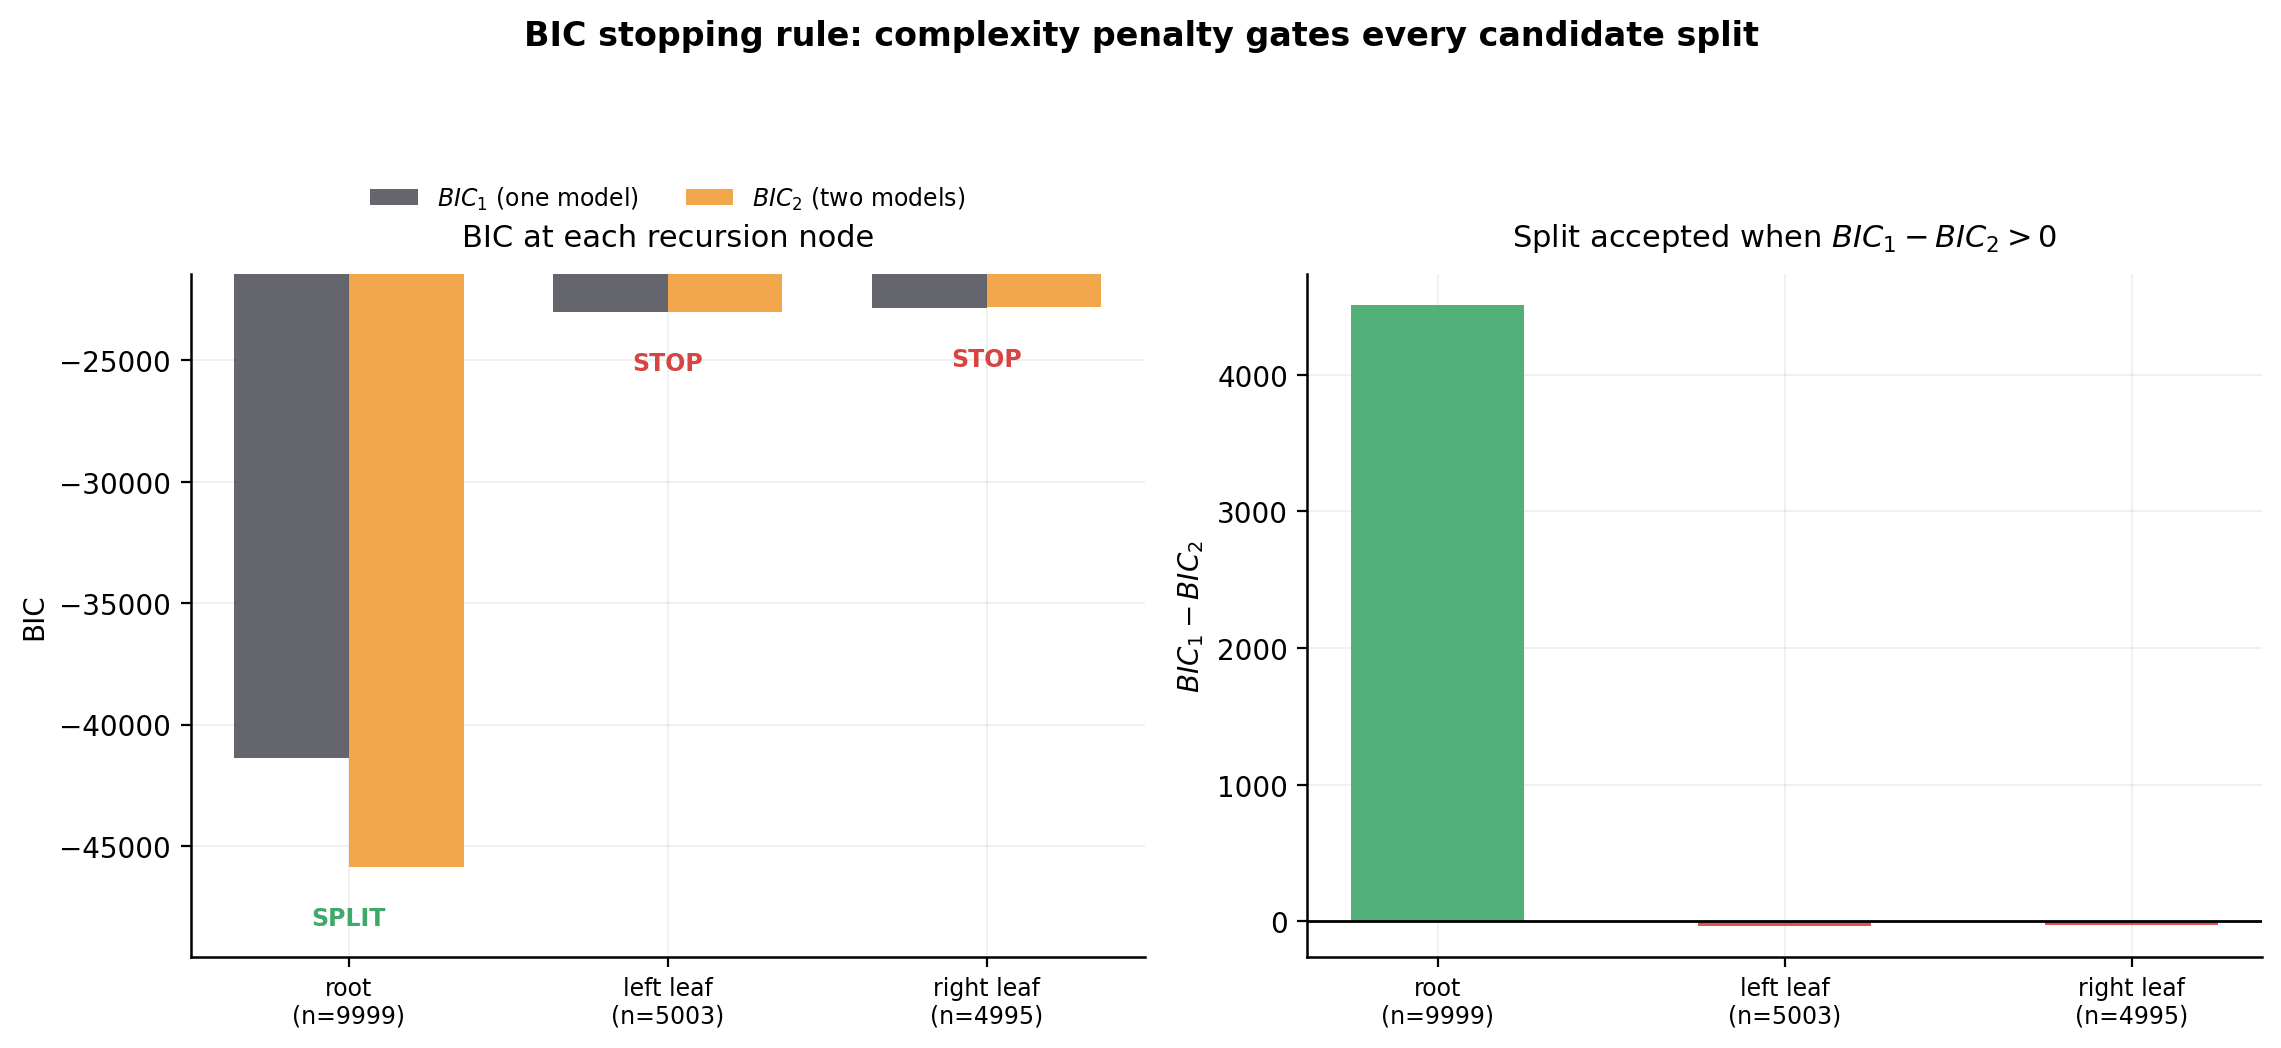
\includegraphics[width=\textwidth]{figs/fig05_bic_gate.png}
    \caption{BIC evaluation at each recursion node.}
    \label{fig:chapter5-5}
\end{figure}

Figure~\ref{fig:chapter5-5} gives the numerical BIC comparison. The root split has
the lower two-model BIC and is accepted, whereas both child splits have higher
two-model BIC values and are rejected.

\begin{figure}[htbp]
    \centering
    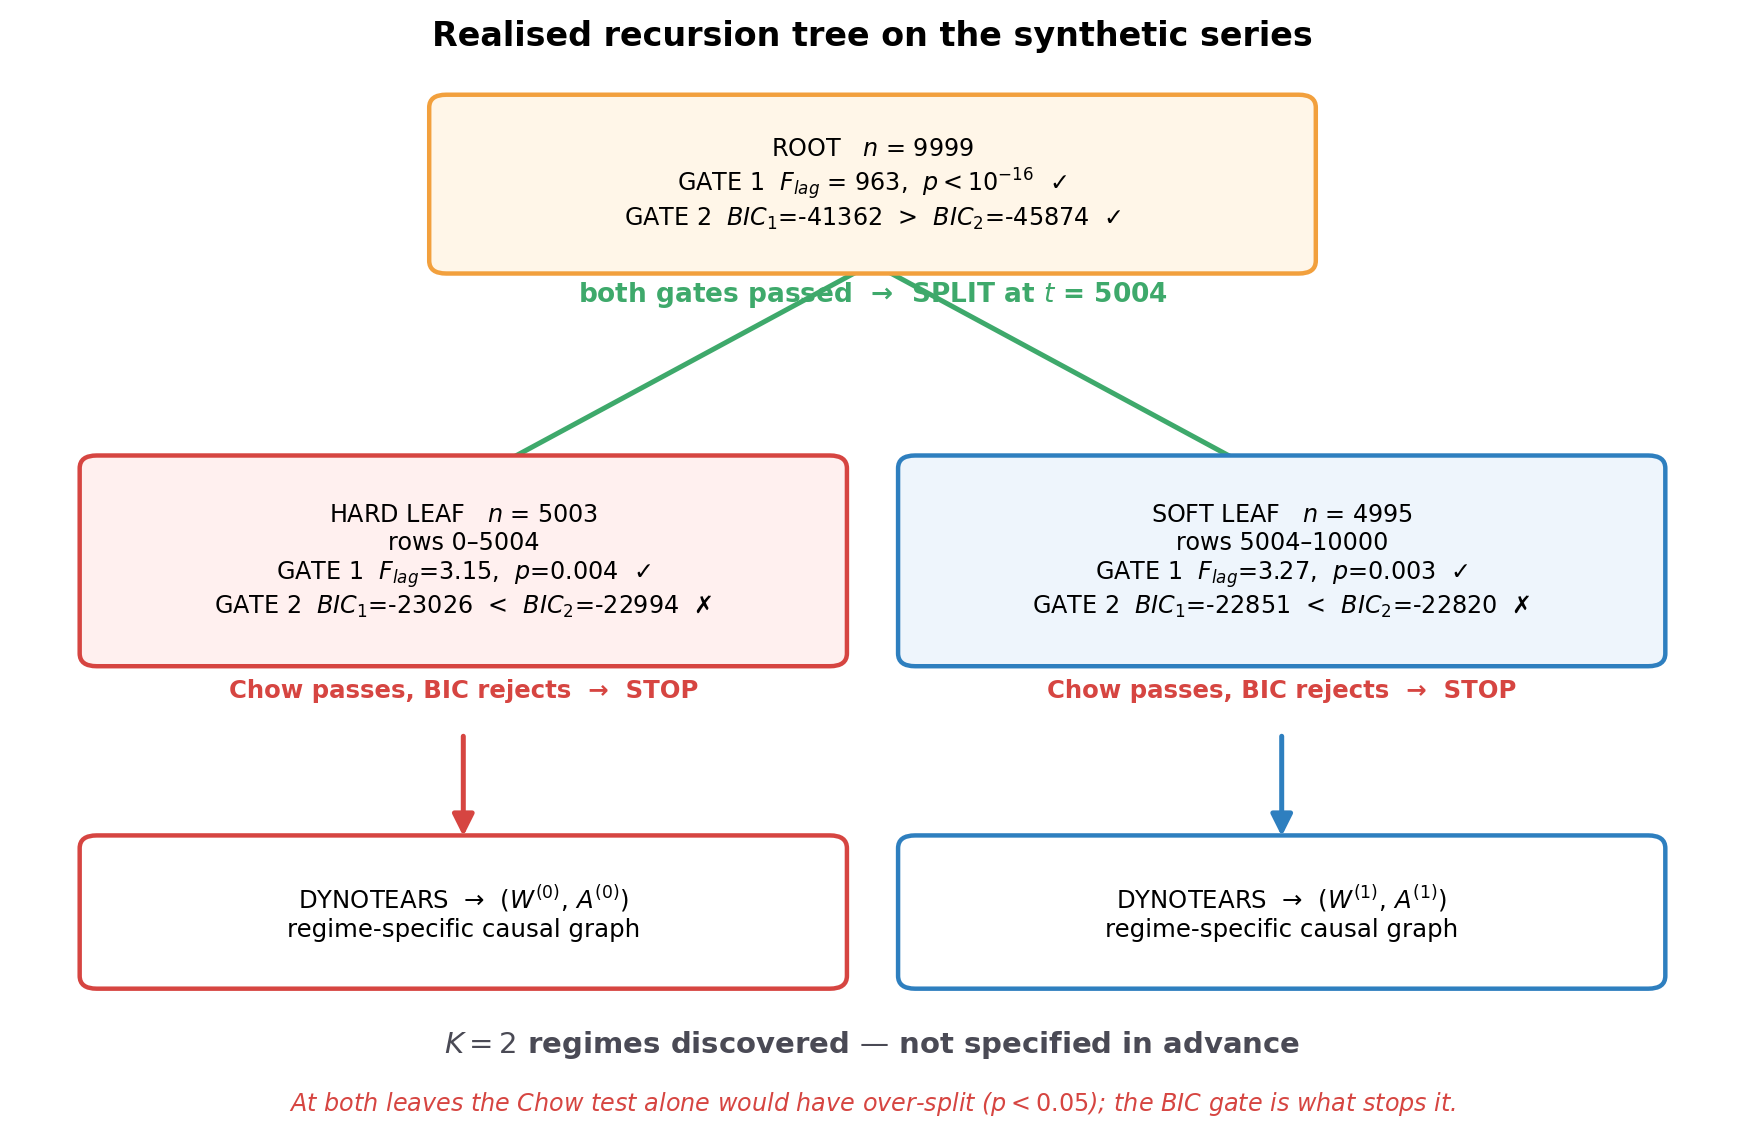
\includegraphics[width=\textwidth]{figs/fig12_recursion_tree.png}
    \caption{Realised recursion tree on the synthetic validation series.}
    \label{fig:chapter5-12}
\end{figure}

Figure~\ref{fig:chapter5-12} presents these decisions as a recursion tree. It shows
the accepted root split, the two terminal leaves, and the subsequent application of
DYNOTEARS. Together, the two figures explain how the final two-regime solution is
formed.


\subsection{Comparison against structure-blind baselines}

$K=2$ regimes are recovered with an Adjusted Rand Index of $0.9984$, without supplying
$K$ in advance. Table~\ref{tab:ch5-regime-recovery} compares this result with
$k$-means, which is given the correct value $K=2$. Even with this advantage,
feature-space clustering fails on three of the four variants.



\begin{table}[htbp]
    \centering
    \small
    \caption{Regime recovery accuracy}
    \label{tab:ch5-regime-recovery}
    \begin{tabularx}{\textwidth}{|>{\raggedright\arraybackslash}X|>{\raggedright\arraybackslash}X|>{\raggedright\arraybackslash}X|}
        \hline
        Method & Basis for grouping & ARI \\ \hline
        \textbf{LIRA (this work)} & causal mechanism invariance, $K$ not supplied & \textbf{0.9984} \\ \hline
        $k$-means, raw features ($K=2$ given) & feature-space proximity & 0.0011 \\ \hline
        $k$-means, standardised features ($K=2$ given) & feature-space proximity & 0.0009 \\ \hline
        $k$-means, rolling means ($K=2$ given, $w=200$) & local level & 0.0112 \\ \hline
        $k$-means, rolling s.d. of $\log F_R$ ($K=2$ given, $w=200$) & local dispersion & 0.5867 \\ \hline
    \end{tabularx}
\end{table}

The result supports the design in Section~5.1.3: the regimes are not separated well
by distributional similarity alone.

The rolling-standard-deviation baseline reaches $\mathrm{ARI}=0.587$. It is included
because the variance of $\log F_R$ differs between regimes. It recovers less than LIRA
and requires $K$ to be supplied in advance.

Figure~\ref{fig:chapter5-8} shows the regime-recovery comparison against the
structure-blind baselines.


\begin{figure}[htbp]
    \centering
    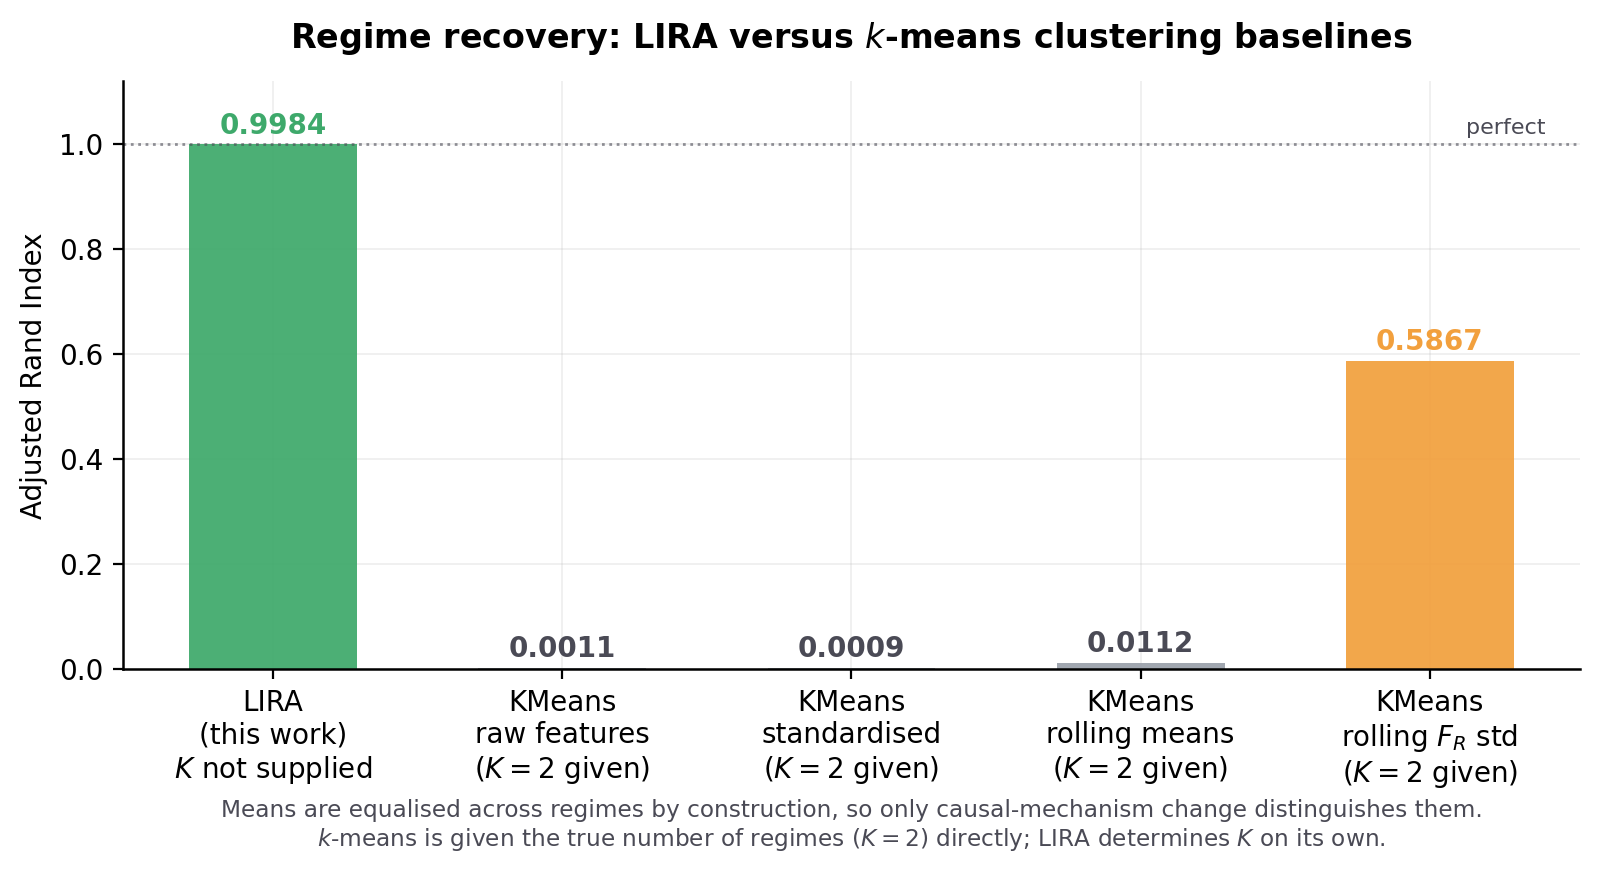
\includegraphics[width=\textwidth]{figs/fig08_baselines.png}
    \caption{Regime recovery: LIRA against structure-blind clustering baselines.}
    \label{fig:chapter5-8}
\end{figure}


\section{Structural coefficient recovery}

Fitting Equation~\eqref{eq:ch4-6} within each leaf recovers the generating coefficients
accurately and identifies the isolated variable in both regimes.

The recovered structural coefficients are reported in Table~\ref{tab:ch5-structural-coefficients}.



\begin{table}[htbp]
    \centering
    \small
    \caption{Recovered structural coefficients}
    \label{tab:ch5-structural-coefficients}
    \begin{tabularx}{\textwidth}{|>{\raggedright\arraybackslash}X|>{\raggedright\arraybackslash}X|>{\raggedright\arraybackslash}X|>{\raggedright\arraybackslash}X|>{\raggedright\arraybackslash}X|>{\raggedright\arraybackslash}X|>{\raggedright\arraybackslash}X|}
        \hline
          & \multicolumn{3}{c|}{Hard State} & \multicolumn{3}{c|}{Soft State} \\ \hline
        Coefficient & True & Recovered & Error & True & Recovered & Error \\ \hline
        $\beta_{L_X}$ & $+0.70$ & $+0.7172$ & $+0.017$ & $+0.18$ & $+0.1830$ & $+0.003$ \\ \hline
        $\beta_{\Gamma}$ & $-0.30$ & $-0.2989$ & $+0.001$ & $+0.20$ & $+0.2030$ & $+0.003$ \\ \hline
        $\beta_{T_{in}}$ & $0.00$ & $+0.0049$ & $+0.005$ & $-0.40$ & $-0.3894$ & $+0.011$ \\ \hline
        $\beta_{HR}$ & $-0.40$ & $-0.4015$ & $-0.002$ & $0.00$ & $-0.0070$ & $-0.007$ \\ \hline
        $\phi$ & $+0.50$ & $+0.4931$ & $-0.007$ & $+0.50$ & $+0.4958$ & $-0.004$ \\ \hline
    \end{tabularx}
\end{table}

The isolated coefficients are $+0.005$ in the Hard State and $-0.007$ in the Soft State.
Both are close to zero and much smaller than the active coefficients. The
autoregressive coefficient is recovered within $0.007$ of its true value.

\textbf{Temporal persistence.} The recovered $\phi$ values of $0.493$ and $0.496$ are
statistically indistinguishable, correctly reflecting that the generating process
assigns identical persistence to both regimes. The framework therefore does not
manufacture a persistence difference where none exists. It should be noted that the
abstract's claim regarding differential temporal persistence across accretion states is
a hypothesis about \textit{real} systems. The present synthetic design does not encode such a
difference, and testing it requires either a generator in which $\phi$ varies by regime
or application to observational data.


\subsection{The pooled-model baseline}

To test whether segmentation is necessary, we fit Equation~\eqref{eq:ch4-6} once
to the full series. The resulting structure matches neither regime.

The pooled and regime-specific estimates are compared in Table~\ref{tab:ch5-pooled}.



\begin{table}[htbp]
    \centering
    \small
    \caption{Pooled model versus regime-specific models}
    \label{tab:ch5-pooled}
    \begin{tabularx}{\textwidth}{|>{\raggedright\arraybackslash}X|>{\raggedright\arraybackslash}X|>{\raggedright\arraybackslash}X|>{\raggedright\arraybackslash}X|}
        \hline
        Coefficient & True (Hard) & True (Soft) & Pooled fit \\ \hline
        $\beta_{L_X}$ & $+0.70$ & $+0.18$ & $+0.2504$ \\ \hline
        $\beta_{\Gamma}$ & $-0.30$ & $+0.20$ & $-0.0285$ \\ \hline
        $\beta_{T_{in}}$ & $0.00$ & $-0.40$ & $-0.1167$ \\ \hline
        $\beta_{HR}$ & $-0.40$ & $0.00$ & $-0.1170$ \\ \hline
        $\phi$ & $+0.50$ & $+0.50$ & $+0.7650$ \\ \hline
    \end{tabularx}
\end{table}

Every coefficient is distorted. The coefficient on $\Gamma$ is negative in one regime
and positive in the other, but the pooled value is almost zero ($-0.029$). Both
isolated variables receive spurious coefficients. The autoregressive coefficient rises
from $0.50$ to $0.765$ because the pooled model attributes between-regime variation
to temporal persistence.

This result shows why a single pooled model can hide the coupling laws of distinct
accretion states.

The recovered and pooled coefficients are compared visually in Figure~\ref{fig:chapter5-7}.


\begin{figure}[htbp]
    \centering
    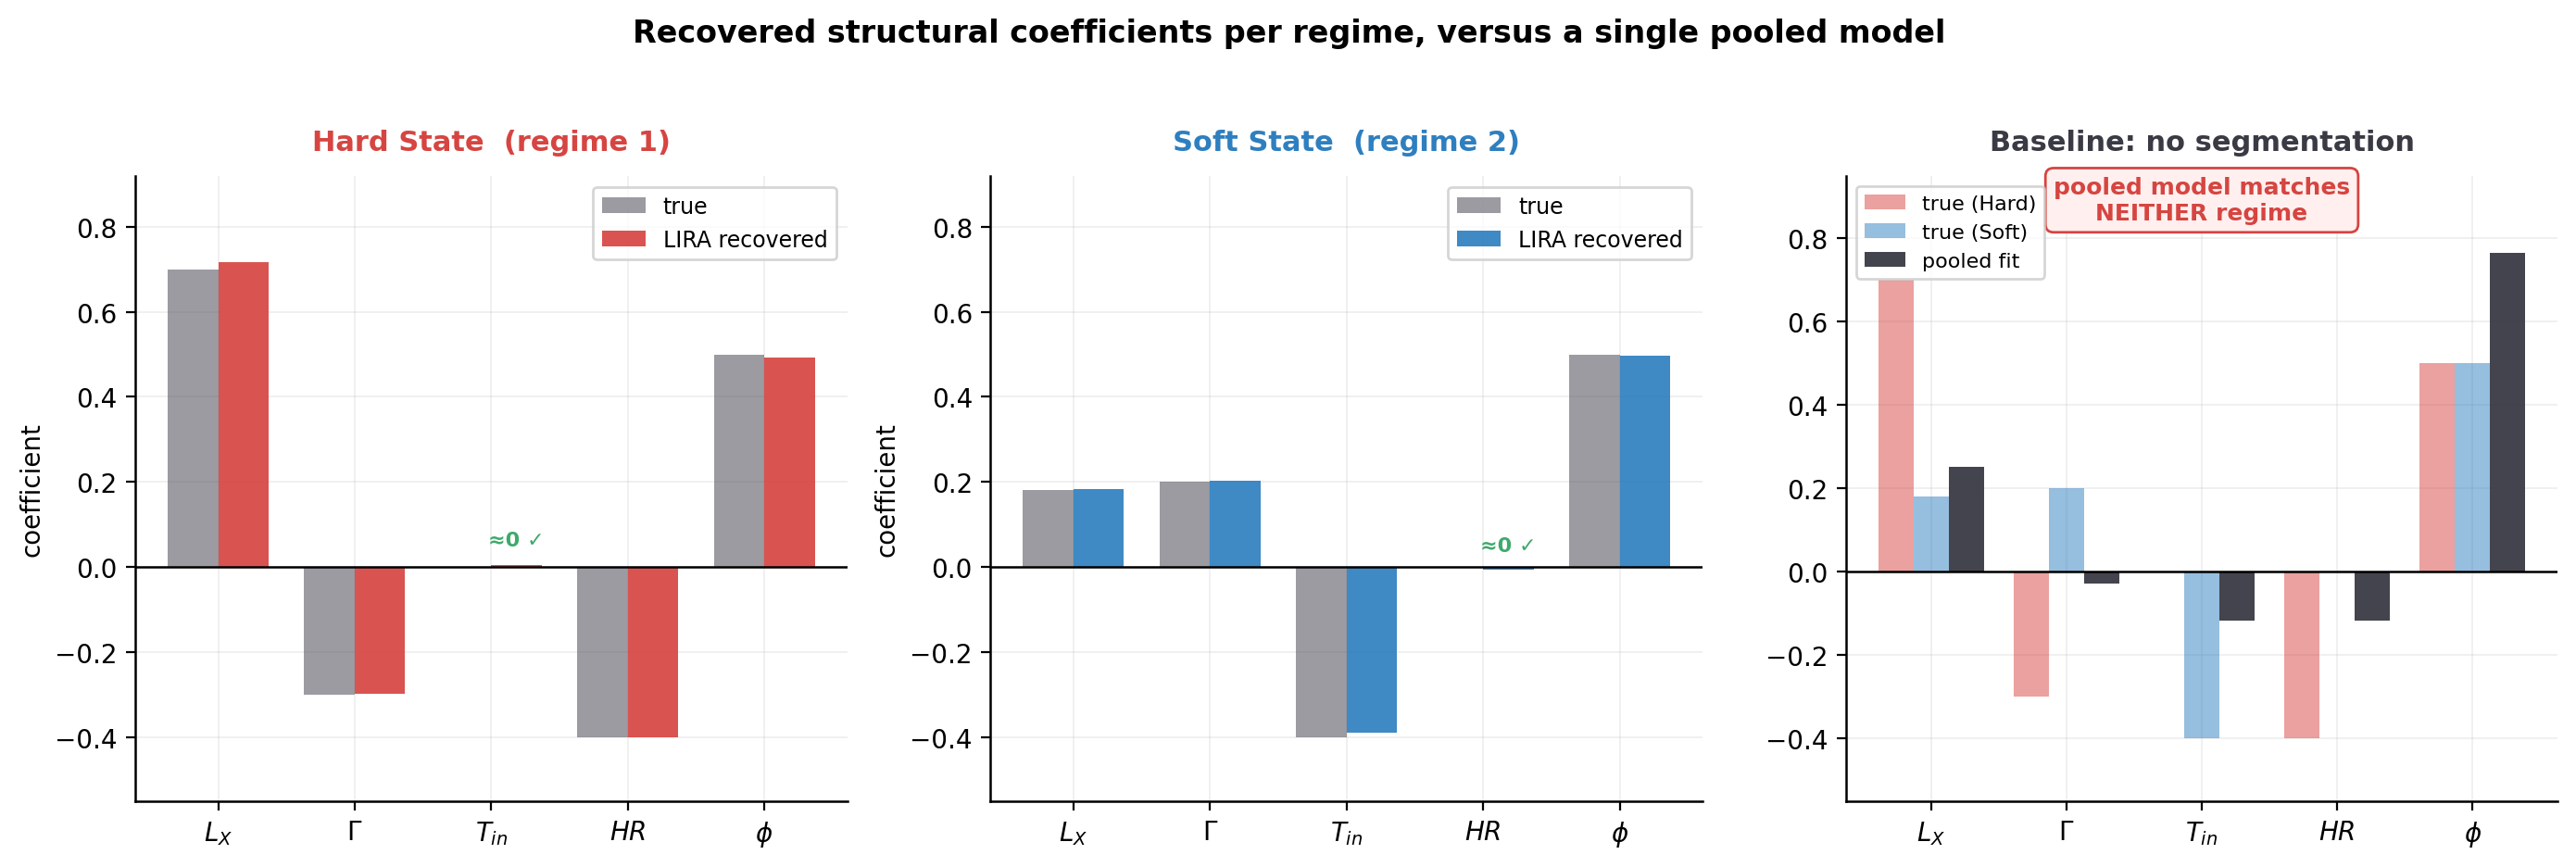
\includegraphics[width=\textwidth]{figs/fig07_coefficients.png}
    \caption{Recovered coefficients per regime, and the pooled model that matches neither.}
    \label{fig:chapter5-7}
\end{figure}


\section{Regime-specific causal graph recovery}

DYNOTEARS applied independently within each discovered leaf recovers the correct graph
structure in both regimes.

The contemporaneous and lagged edge estimates are reported in Tables~\ref{tab:ch5-contemporaneous}
and~\ref{tab:ch5-lagged}, respectively.



\begin{table}[htbp]
    \centering
    \small
    \caption{Contemporaneous edge recovery ($\hat{W}$)}
    \label{tab:ch5-contemporaneous}
    \begin{tabularx}{\textwidth}{|>{\raggedright\arraybackslash}X|>{\raggedright\arraybackslash}X|>{\raggedright\arraybackslash}X|>{\raggedright\arraybackslash}X|>{\raggedright\arraybackslash}X|}
        \hline
        Edge & Hard: true & Hard: $\hat{W}$ & Soft: true & Soft: $\hat{W}$ \\ \hline
        $L_X \to F_R$ & present $(+)$ & $+0.315$ yes & present $(+)$ & $+0.079$ yes \\ \hline
        $\Gamma \to F_R$ & present $(-)$ & $-0.100$ yes & present $(+)$ & $+0.090$ yes \\ \hline
        $T_{in} \to F_R$ & \textbf{absent} & \textbf{absent} yes & present $(-)$ & $-0.212$ yes \\ \hline
        $HR \to F_R$ & present $(-)$ & $-0.157$ yes & \textbf{absent} & \textbf{absent} yes \\ \hline
        any edge into $L_X$ & absent & absent yes & absent & absent yes \\ \hline
\end{tabularx}
\end{table}

Table~\ref{tab:ch5-contemporaneous} confirms the contemporaneous structure. The
active edges have the correct signs, the state-specific isolated variable is absent,
and $L_X$ has no contemporaneous parent.



\begin{table}[htbp]
    \centering
    \small
    \caption{Lagged edge recovery ($\hat{A}$, self-lags)}
    \label{tab:ch5-lagged}
    \begin{tabularx}{\textwidth}{|>{\raggedright\arraybackslash}X|>{\raggedright\arraybackslash}X|>{\raggedright\arraybackslash}X|>{\raggedright\arraybackslash}X|}
        \hline
        Self-lag & True & Hard: $\hat{A}$ & Soft: $\hat{A}$ \\ \hline
        $L_X$ & $0.90$ & $0.851$ & $0.851$ \\ \hline
        $\Gamma$ & $0.90$ & $0.854$ & $0.839$ \\ \hline
        $T_{in}$ & $0.90$ & $0.843$ & $0.838$ \\ \hline
        $HR$ & $0.90$ & $0.854$ & $0.847$ \\ \hline
        $F_R$ & $0.50$ & $0.527$ & $0.495$ \\ \hline
\end{tabularx}
\end{table}

Table~\ref{tab:ch5-lagged} reports the temporal self-lags. The four spectral
variables are recovered close to the generating value of $0.90$, while the radio
luminosity self-lag is close to $0.50$. Thus, the method recovers temporal dependence
as well as contemporaneous edges.

All edge signs are correct, the isolated variable is excluded in each regime, and
$L_X$ has no parent other than its own lag. The edge magnitudes are smaller than the
generating coefficients because of $L_1$ soft-thresholding. This does not change the
structural conclusions; unbiased effect magnitudes are estimated in Section~5.6.


\begin{figure}[htbp]
    \centering
    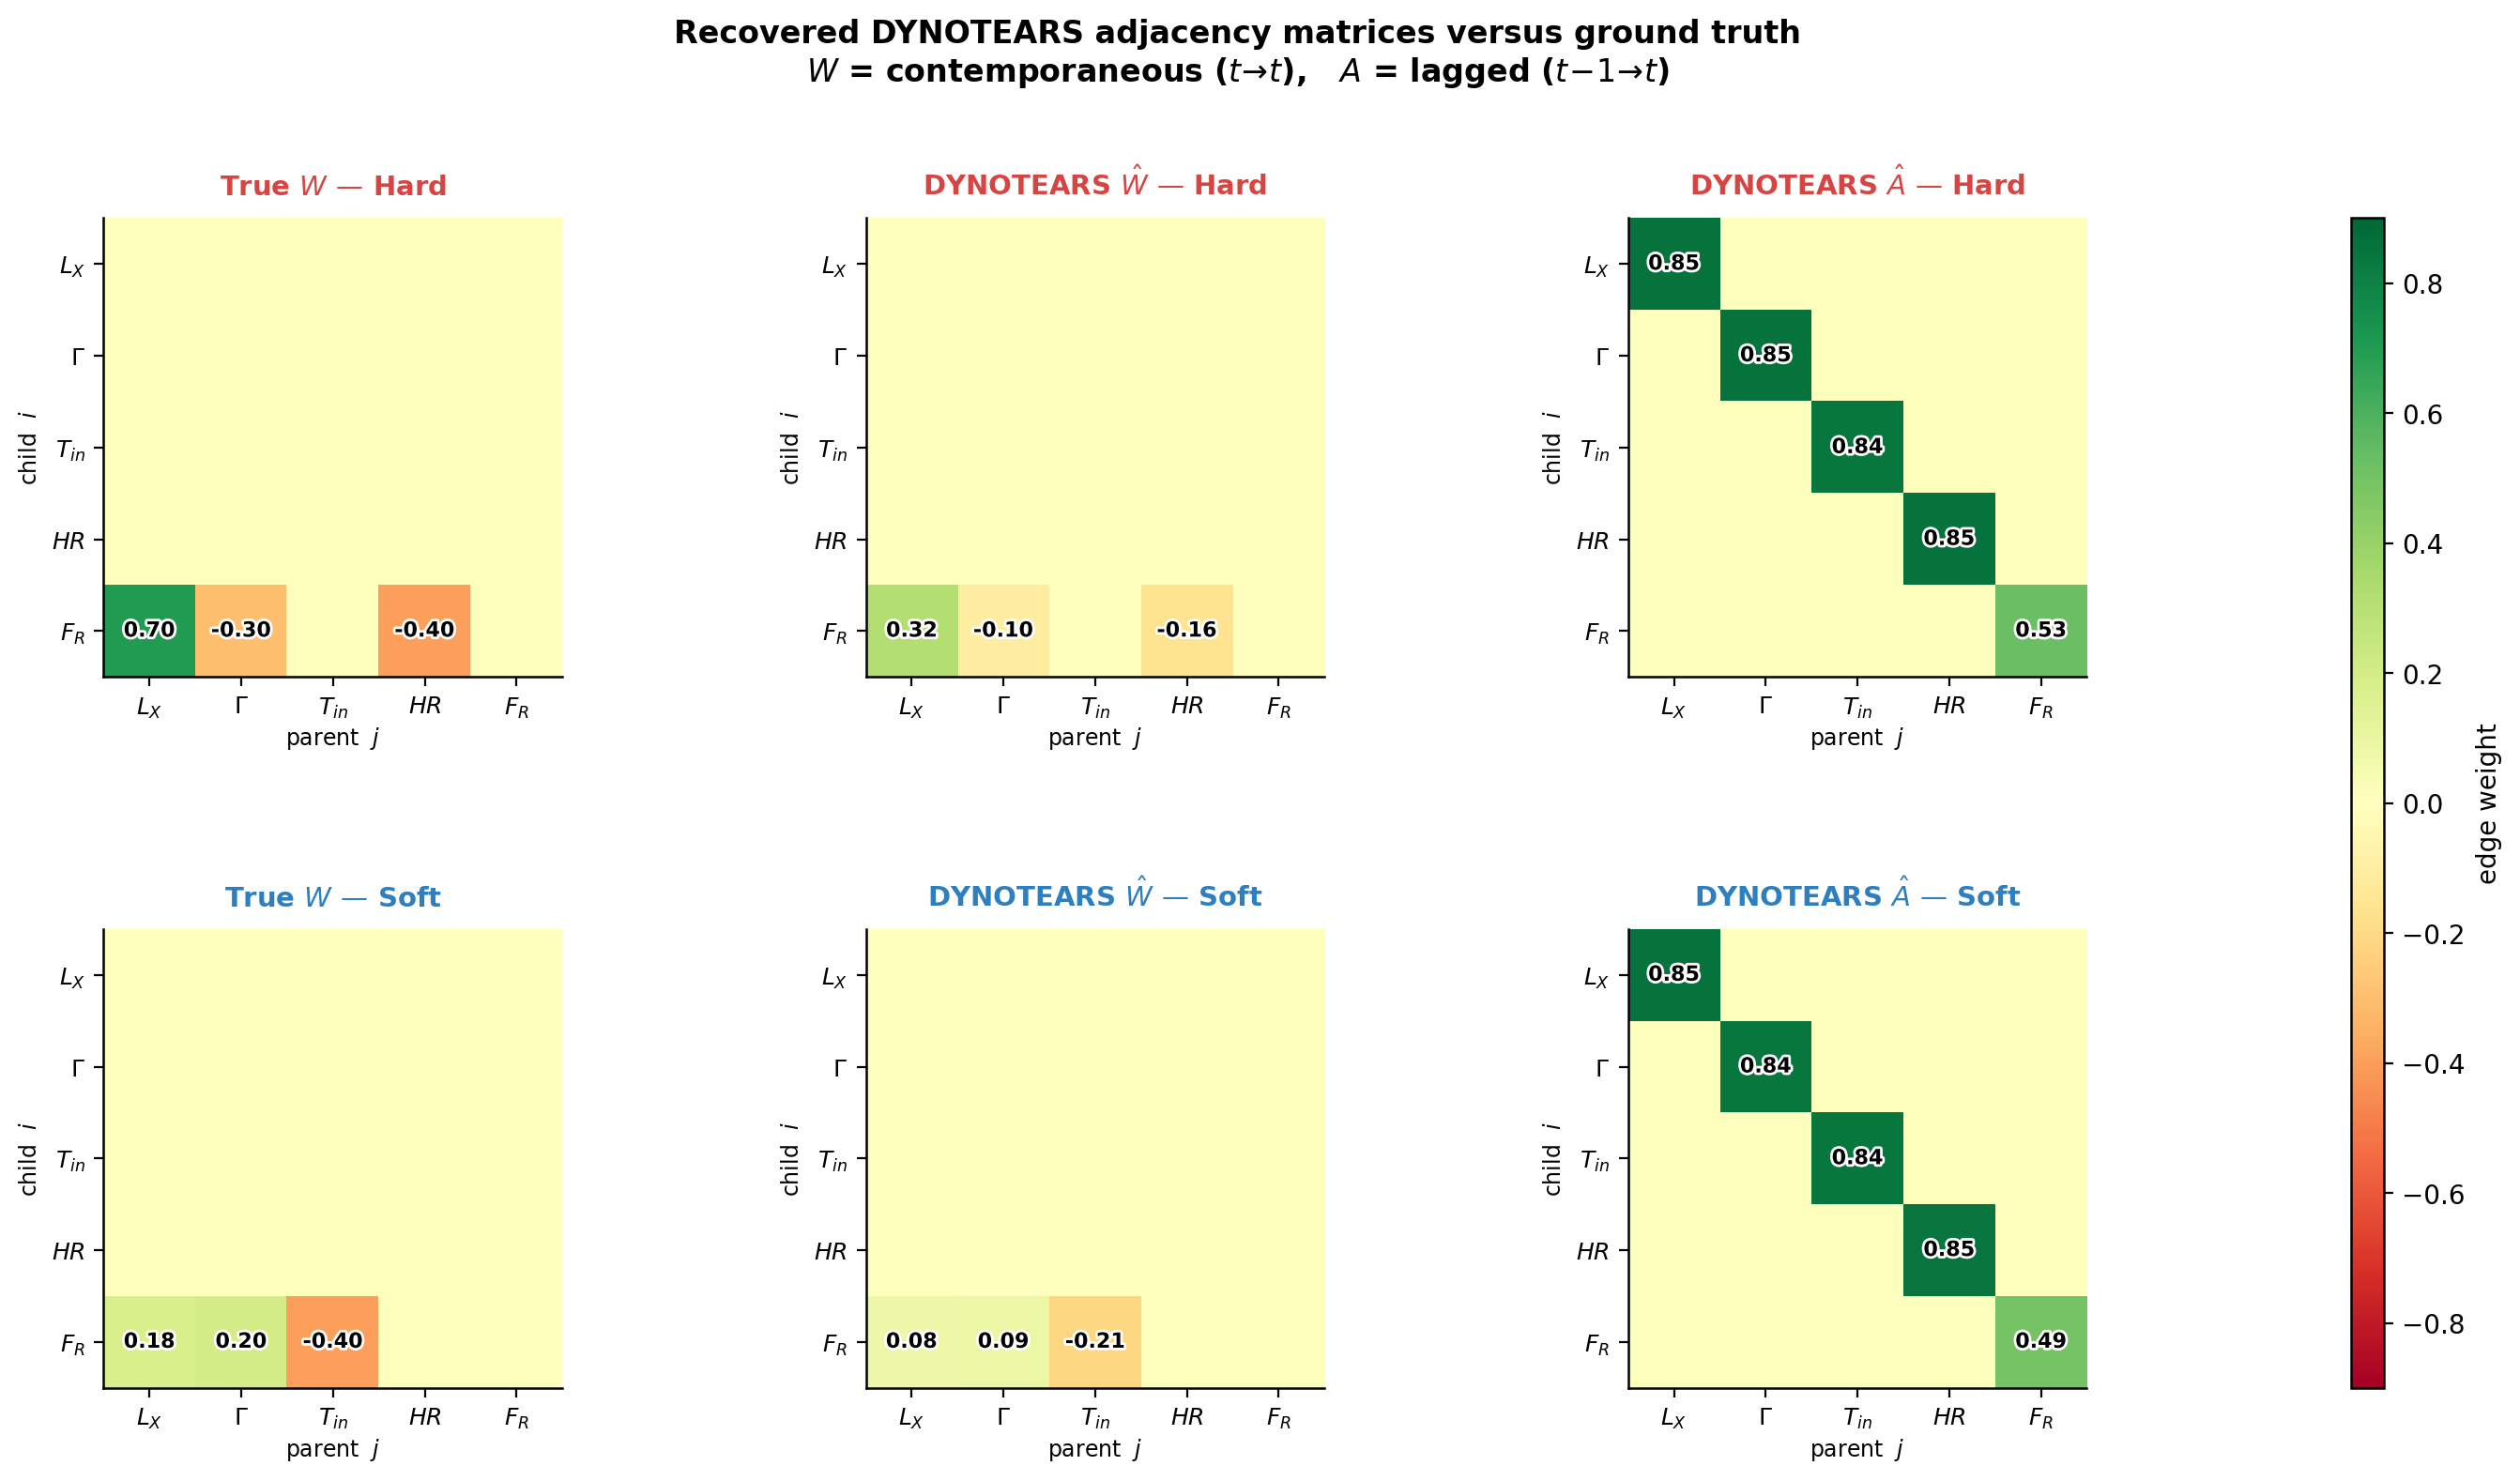
\includegraphics[width=\textwidth]{figs/fig09_adjacency.png}
    \caption{Recovered adjacency matrices against ground truth, for both the contemporaneous and lagged components.}
    \label{fig:chapter5-9}
\end{figure}

Figure~\ref{fig:chapter5-9} shows the same comparison in matrix form. The left
column is the true contemporaneous matrix $W$ for each regime. The middle column is
the recovered matrix $\hat{W}$, and the right column is the recovered lagged matrix
$\hat{A}$. In the Hard State the truth has three edges into $F_R$ and the recovery
selects the same three cells. In the Soft State the three active cells are different
and again all three are selected. The cells that are zero in the truth stay zero in
the recovery. The recovered edge weights are smaller than the true ones because of
the $L_1$ soft-thresholding in Stage 2. The lagged matrices are diagonal, so only
self-lags appear, and their entries are close to the generating values given in
Table~\ref{tab:ch5-lagged}. The pattern of edges, the signs of the edges, and the
isolated variable are therefore correct in both regimes.


\section{Causal effect estimation and validation}


\subsection{Effect estimates}

Backdoor adjustment with the remaining parents gives more accurate effect estimates
than the penalised Stage 2 weights, as expected from Section~4.8.

The estimated causal effects are listed in Table~\ref{tab:ch5-effects}.



\begin{table}[htbp]
    \centering
    \footnotesize
    \setlength{\tabcolsep}{4pt}
    \renewcommand{\arraystretch}{1.3}
    \caption{Estimated causal effects, refutation outcomes, and robustness}
    \label{tab:ch5-effects}
    \begin{tabularx}{\textwidth}{|>{\raggedright\arraybackslash}p{1.3cm}|>{\raggedright\arraybackslash}p{1.5cm}|>{\centering\arraybackslash}X|>{\centering\arraybackslash}X|>{\centering\arraybackslash}X|>{\centering\arraybackslash}X|>{\centering\arraybackslash}X|>{\centering\arraybackslash}X|}
        \hline
        Regime & Treatment & Estimate & True & \makecell{Random\\c.c.} & Placebo & Subset & Robustness \\ \hline
        Hard & $L_X$ & $+0.7111$ & $+0.70$ & $+0.7110$ & $+0.0016$ & $+0.7116$ & $+0.680$ \\ \hline
        Hard & $\Gamma$ & $-0.2964$ & $-0.30$ & $-0.2964$ & $-0.0003$ & $-0.2963$ & $+0.473$ \\ \hline
        Hard & $HR$ & $-0.3981$ & $-0.40$ & $-0.3981$ & $+0.0011$ & $-0.3985$ & $+0.556$ \\ \hline
        Hard & $F_R(t{-}1)$ & $+0.4983$ & $+0.50$ & $+0.4983$ & $-0.0006$ & $+0.4979$ & $+0.734$ \\ \hline
        Soft & $L_X$ & $+0.1799$ & $+0.18$ & $+0.1800$ & $-0.0006$ & $+0.1800$ & $+0.325$ \\ \hline
        Soft & $\Gamma$ & $+0.1994$ & $+0.20$ & $+0.1993$ & $-0.0005$ & $+0.1999$ & $+0.338$ \\ \hline
        Soft & $T_{in}$ & $-0.3833$ & $-0.40$ & $-0.3833$ & $-0.0001$ & $-0.3829$ & $+0.515$ \\ \hline
        Soft & $F_R(t{-}1)$ & $+0.5062$ & $+0.50$ & $+0.5063$ & $-0.0007$ & $+0.5059$ & $+0.728$ \\ \hline
    \end{tabularx}
\end{table}

Every estimate is within $0.017$ of its generating value. The random common-cause and
subset tests leave the estimates almost unchanged, while the placebo test reduces
every effect to within $0.002$ of zero.

The effect estimates and refutation outcomes are visualised in Figure~\ref{fig:chapter5-10}.

\begin{figure}[htbp]
    \centering
    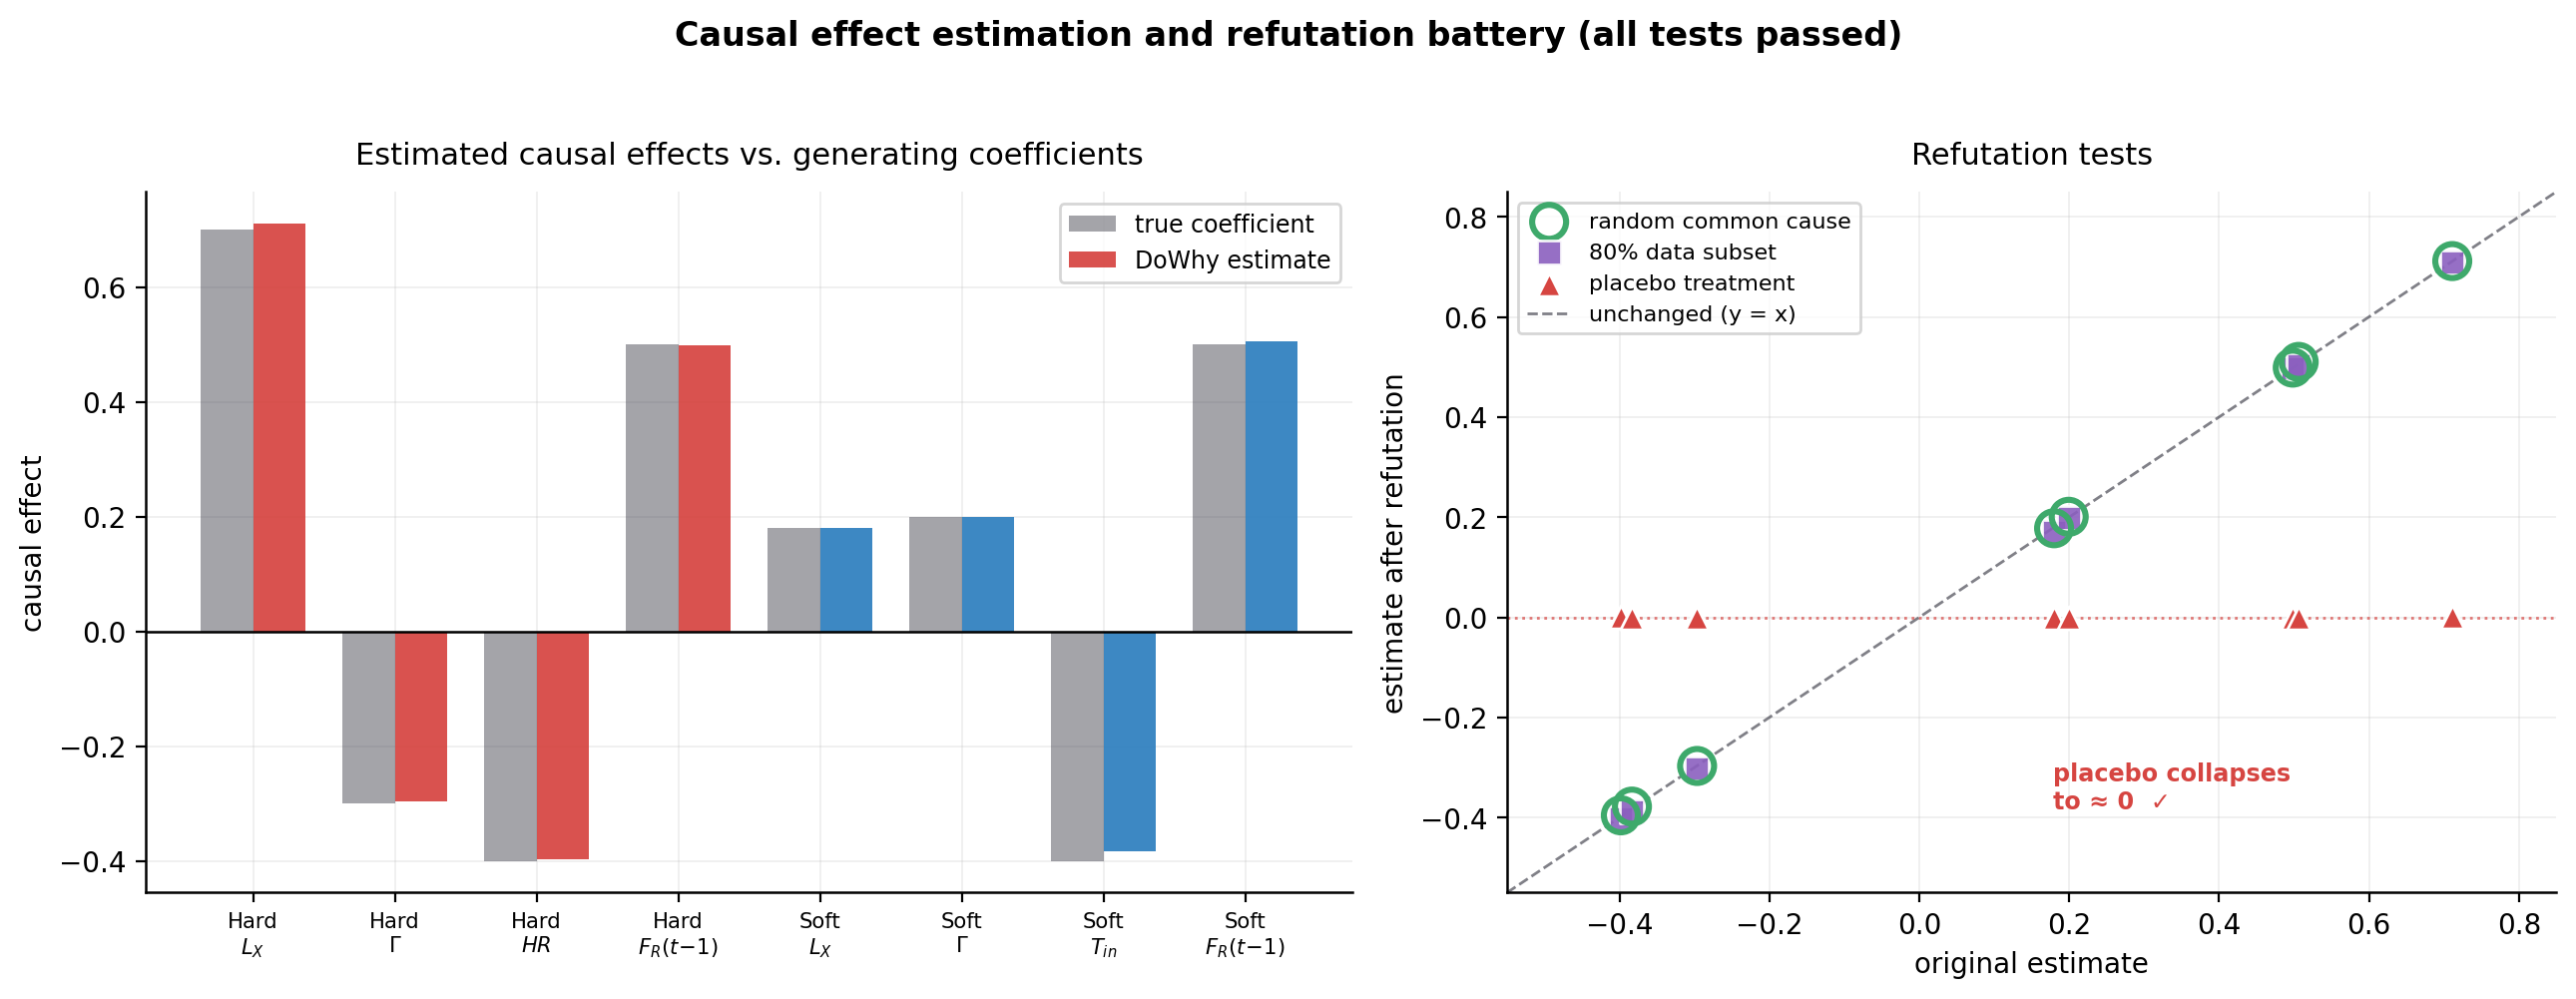
\includegraphics[width=\textwidth]{figs/fig10_effects_refutation.png}
\caption{Causal effect estimation and refutation battery. All reported tests pass.}
    \label{fig:chapter5-10}
\end{figure}

Figure~\ref{fig:chapter5-10} visualises these results. The left panel pairs each
estimated effect with the generating coefficient that produced it. The grey bar is
the true coefficient and the coloured bar is the estimate. The two bars have almost
the same height for every treatment. The right panel shows the three refutation
tests. Each point plots an estimate before refutation against the same estimate
after refutation. The random common-cause and subset points fall on the dashed
diagonal, so those refuters left the estimates unchanged. The placebo points fall on
the zero line instead, so the placebo treatment drove the estimate to zero. All
tests therefore pass.


\subsection{Sensitivity to unobserved confounding}

The Cinelli--Hazlett robustness value is the minimum residual variance that an
unobserved confounder must explain in both the treatment and the outcome to reduce an effect
to zero. Robustness increases with effect magnitude, with Pearson correlation
$r=0.888$. The weaker Soft State effects are therefore more sensitive to hidden
confounding and require more cautious interpretation.

\begin{figure}[htbp]
    \centering
    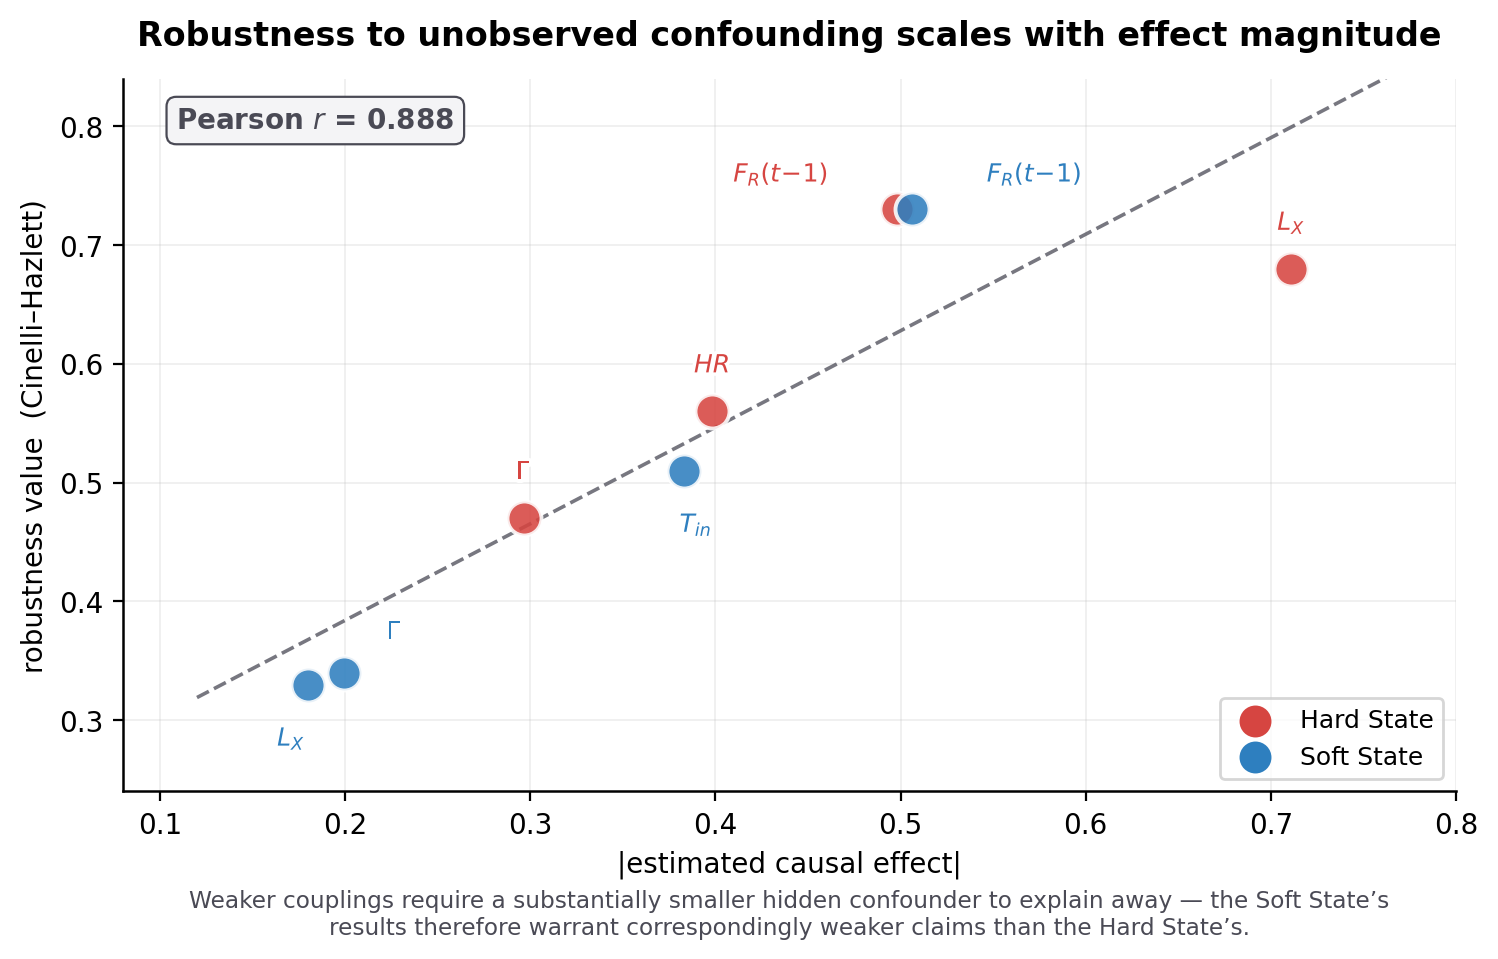
\includegraphics[width=\textwidth]{figs/fig11_robustness.png}
    \caption{Robustness to unobserved confounding as a function of estimated causal-effect magnitude.}
    \label{fig:chapter5-11}
\end{figure}

Figure~\ref{fig:chapter5-11} plots all eight effects of Table~\ref{tab:ch5-effects}
together. The horizontal axis gives the magnitude of each estimated effect and the
vertical axis gives its robustness value. Red points are Hard State effects and blue
points are Soft State effects. The points rise from the lower left to the upper
right. The dashed line is the linear fit through the points and the text box gives
the Pearson correlation of $r=0.888$. The two lowest points belong to the Soft
State $L_X$ and $\Gamma$ couplings. Their robustness values are near $0.33$, so a
confounder would have to explain about a third of the residual variance in both the
treatment and the outcome to erase them. The $F_R$ lag effects reach the highest
robustness values of $0.73$. The largest single effect, the Hard State $L_X$ coupling
at $0.71$, follows closely with $0.68$. An unobserved confounder would therefore have
to be strong to remove any of the eight effects. The weaker Soft State couplings need
the most caution because they can be removed by the weakest confounders.

\subsection{Graph falsification}

Falsification testing compares the conditional-independence implications of each
recovered DAG with randomly permuted graphs. With 20 permutations, neither DAG is
rejected at $\alpha=0.05$. One permutation falls within the Markov equivalence class
for each regime. The Hard State graph violates 15 of 22 local Markov conditions and
the Soft State graph violates 10 of 22; both outperform 95\% of the alternatives.

The falsification results are summarised in Table~\ref{tab:ch5-falsification}.

\begin{table}[htbp]
    \centering
    \small
    \caption{Graph falsification summary}
    \label{tab:ch5-falsification}
    \begin{tabularx}{\textwidth}{|>{\raggedright\arraybackslash}X|>{\centering\arraybackslash}X|>{\centering\arraybackslash}X|>{\centering\arraybackslash}X|>{\centering\arraybackslash}X|>{\raggedright\arraybackslash}X|}
        \hline
        Regime & LMC violations & Better than & Permutations in MEC & $p$ & Verdict \\ \hline
        Hard & 15 / 22 & 95.0\% & 1 / 20 & 0.05 & not rejected \\ \hline
        Soft & 10 / 22 & 95.0\% & 1 / 20 & 0.05 & not rejected \\ \hline
    \end{tabularx}
\end{table}

\textbf{Limitation.} With only 20 permutations, the $p$-value is restricted to
multiples of 0.05. The result is therefore indicative rather than conclusive. At
least 100 permutations should be used before publication.

\section{Summary of validation outcomes}

Table~\ref{tab:ch5-summary} consolidates the main validation outcomes.

\begin{table}[htbp]
    \centering
    \small
    \caption{Summary of experimental findings}
    \label{tab:ch5-summary}
    \begin{tabularx}{\textwidth}{|>{\raggedright\arraybackslash}p{3.4cm}|>{\raggedright\arraybackslash}X|>{\raggedright\arraybackslash}p{2.5cm}|}
        \hline
        Claim & Evidence & Outcome \\ \hline
        AR(1) term restores residual independence & Ljung--Box $p$: $<10^{-16} \to 0.211$ & confirmed (Section~5.2) \\ \hline
        Boundary is localised accurately & $\tau^* = 5004$ vs. true $5000$ & confirmed (Section~5.3.1) \\ \hline
        $K$ is determined automatically & $K = 2$ recovered, not specified & confirmed (Section~5.3.2) \\ \hline
        Both gates are necessary & Chow passes at both leaves, BIC rejects & confirmed (Section~5.3.2) \\ \hline
        Regimes are not separable by feature distribution & $k$-means (given $K=2$) ARI $\leq 0.012$ for three of four variants versus LIRA $0.998$ & confirmed (Section~5.3.3) \\ \hline
        Coefficients are recovered accurately & Maximum error $0.017$ across both regimes & confirmed (Section~5.4) \\ \hline
        Pooling produces a spurious structure & $\beta_\Gamma$ averaged to $-0.029$, $\phi$ inflated to $0.765$ & confirmed (Section~5.4.1) \\ \hline
        Regime-specific graphs are recovered & All signs correct, isolated variable excluded in each & confirmed (Section~5.5) \\ \hline
        Effects survive refutation & Placebo $<0.002$, other estimates unchanged & confirmed (Section~5.6.1) \\ \hline
        Robustness scales with effect size & $r = 0.888$ & confirmed (Section~5.6.2) \\ \hline
        Recovered graphs are not falsified & Neither rejected at $\alpha=0.05$ & indicative only (Section~5.6.3) \\ \hline
    \end{tabularx}
\end{table}

The table gives a compact view of the whole validation study. Each row states one
claim, the supporting evidence, and the section where the evidence is produced. Ten
of the eleven claims are confirmed by the experiments. The falsification claim is
marked indicative only because the test used 20 permutations. The other rows show
that every stage of the pipeline produced the expected result, from residual
cleaning to effect estimation.
